% =======================================================
% Arquivo Principal do TCC - Joaquim Walisson
% Baseado no template abntex2 UFC
% =======================================================

\documentclass[        
    a4paper,          % Tamanho da folha A4
    12pt,             % Tamanho da fonte 12pt
    chapter=TITLE,    % Todos os capitulos devem ter caixa alta
    section=Title,    % Todas as secoes devem ter caixa alta somente na primeira letra
    subsection=Title, % Todas as subsecoes devem ter caixa alta somente na primeira letra
    oneside,          % Usada para impressao em apenas uma face do papel
    english,          % Hifenizacoes em ingles
    spanish,          % Hifenizacoes em espanhol
    brazil,           % Ultimo idioma eh o idioma padrao do documento
    fleqn             % Equacoes alinhadas a esquerda
]{abntex2}

% Importações de pacotes
\usepackage[utf8]{inputenc}                         % Acentuação direta
\usepackage[T1]{fontenc}                            % Codificação da fonte em 8 bits
\usepackage{graphicx}                               % Inserir figuras
\usepackage{amsfonts, amssymb, amsmath}             % Fonte e símbolos matemáticos
\usepackage{booktabs}                               % Comandos para tabelas
\usepackage{verbatim}                               % Texto é interpretado como escrito no documento
\usepackage{multirow, array}                        % Múltiplas linhas e colunas em tabelas
\usepackage{indentfirst}                            % Endenta o primeiro parágrafo de cada seção
\usepackage{listings}                               % Utilizar código-fonte no documento
\usepackage{xcolor}
\usepackage[portuguese,ruled,lined]{algorithm2e}    % Escrever algoritmos
\usepackage{algorithmic}                            % Criar algoritmos
\usepackage{amsgen}
\usepackage{lipsum}                                 % Usar a simulação de texto Lorem Ipsum
%\usepackage{titlesec}                              % Permite alterar os títulos do documento
\usepackage{tocloft}                                % Permite alterar a formatação do Sumário
\usepackage{etoolbox}                               % Usado para alterar a fonte da Section no Sumário
\usepackage[acronym,nogroupskip,nonumberlist]{glossaries}   % Permite fazer o glossário

\usepackage[font=singlespacing,format=plain,justification=justified,skip=0pt,singlelinecheck=false]{caption} % Altera o comportamento da tag caption

\usepackage[alf, abnt-emphasize=bf, recuo=0cm, abnt-etal-cite=2, abnt-etal-list=0, abnt-etal-text=it]{abntex2cite}  % Citações padrão ABNT
%\usepackage[bottom]{footmisc}                      % Mantém as notas de rodapé sempre na mesma posição
%\usepackage{times}                                 % Usa a fonte Times
%%%%%%%%%%%%%%%%%%% AVISO %%%%%%%%%%%%%%%%%%%%%%%%%%%%%%%%%%%%%%%%
% Descomente as duas linhas abaixo para alterar o texto de Times New Roman para Arial:
%\usepackage{helvet}
%\renewcommand{\familydefault}{\sfdefault}          % Usa a fonte Arial
%%%%%%%%%%%%%%%%%%%%%%%%%%%%%%%%%%%%%%%%%%%%%%%%%%%%%%%%%%%%%%%%%%

\usepackage{mathptmx}         % Usa a fonte Times New Roman
%\usepackage{lmodern}         % Usa a fonte Latin Modern
%\usepackage{subfig}          % Posicionamento de figuras
%\usepackage{scalefnt}        % Permite redimensionar tamanho da fonte
%\usepackage{color, colortbl} % Comandos de cores
%\usepackage{lscape}          % Permite páginas em modo "paisagem"
%\usepackage{ae, aecompl}     % Fontes de alta qualidade
%\usepackage{picinpar}        % Dispor imagens em parágrafos
%\usepackage{latexsym}        % Símbolos matemáticos
%\usepackage{upgreek}         % Fonte letras gregas
\usepackage{appendix}         % Gerar o apêndice no final do documento
\usepackage{paracol}          % Criar parágrafos sem indentação
\usepackage{lib/ufctex}       % Biblioteca com as normas da UFC para trabalhos acadêmicos
\usepackage{pdfpages}         % Incluir PDF no documento
\usepackage{float}
\usepackage{placeins}
\usepackage{needspace}
\usepackage{microtype}        % Melhora justificação e reduz linhas curtas (carregado após a fonte)

% ====================================================================
% Ajustes globais de diagramação (sempre após lib/ufctex)
% ====================================================================
\clubpenalty=10000            % Evita linha órfã (1ª linha isolada no fim da página)
\widowpenalty=10000           % Evita linha viúva (última linha isolada no topo da página)
\displaywidowpenalty=10000    % Evita viúva após equações em destaque
\finalhyphendemerits=10000    % Desencoraja hifenização na penúltima linha do parágrafo
\raggedbottom                 % Evita "esticar" espaços verticais entre parágrafos

\makeglossaries % Organiza e gera a lista de abreviaturas, símbolos e glossário
\makeindex      % Gera o índice do documento
\setlength{\mathindent}{0pt} 

% --- Nível do Trabalho ---
\trabalhoacademico{tccgraduacao}
\ehqualificacao{nao}
\removerbordasdohyperlink{sim} 
%\cordohyperlink{nao}

% --- Informações da Instituição ---
\ies{Universidade Federal do Ceará}
\iessigla{UFC}
\centro{Campus Sobral}
\departamento{Curso de Engenharia da Computação}
\graduacaoem{Engenharia da Computação}
\habilitacao{bacharel} 

% --- Informações do Trabalho ---
\autor{Joaquim Walisson Portela de Sousa}
\titulo{Desenvolvimento Web para Mapas Digitais: \\ Aplicação no Projeto Sobral em Mapas}
\data{2025}
\local{Sobral}
\dataaprovacao{} % Preencher quando tiver a data da defesa

% --- Orientação ---
\orientador{Prof. Dr. Iális Cavalcante de Paula Júnior}
\orientadories{Universidade Federal do Ceará (UFC)}
\orientadorcentro{Campus Sobral}
\orientadorfeminino{nao} 

\coorientador{} % Deixe em branco se não houver

% --- Banca Examinadora ---
% Atualize os nomes quando a banca for definida. Deixe em branco para remover a linha.
\membrodabancadois{Prof. Dr. Nome do Membro Dois}
\membrodabancadoiscentro{Curso de Engenharia da Computação}
\membrodabancadoisies{Universidade Federal do Ceará (UFC)}

\membrodabancatres{Prof. Me. Nome do Membro Três}
\membrodabancatrescentro{Curso de Engenharia da Computação}
\membrodabancatresies{Universidade Federal do Ceará (UFC)}

% =======================================================
% INÍCIO DO DOCUMENTO
% =======================================================
\begin{document}    

    % --- Pré-textuais ---
    \imprimircapa
    \imprimirfolhaderosto{}
    %\imprimirfichacatalografica{1-pre-textuais/ficha-catalografica} % Descomente após a biblioteca gerar a ficha
    \imprimirfolhadeaprovacao
    
    \imprimirdedicatoria{1-pre-textuais/dedicatoria}
    \imprimiragradecimentos{1-pre-textuais/agradecimentos}
    \imprimirepigrafe{1-pre-textuais/epigrafe}
    
    \imprimirresumo{1-pre-textuais/resumo}
    \imprimirabstract{1-pre-textuais/abstract}
    
    \renewcommand*\listfigurename{Lista de Figuras}
    \imprimirlistadeilustracoes
    %\imprimirlistadetabelas
    %\imprimirlistadecodigosfonte
    \imprimirlistadeabreviaturasesiglas
    %\imprimirlistadesimbolos{1-pre-textuais/lista-de-simbolos}   
    \imprimirsumario
    
    \setcounter{table}{0}
    
    % --- Textuais ---
    \textual
    \chapter{Introdução}
\label{cap:introducao}

A crescente complexidade da gestão urbana moderna exige que a Administração Pública adote infraestruturas tecnológicas capazes de processar, organizar e democratizar o acesso a grandes volumes de dados geoespaciais do município. Nesse cenário, os Sistemas de Informação Geográfica (SIG), do inglês \textit{Geographic Information System} (GIS), baseados na \textit{web} (WebGIS), consolidaram-se como ferramentas essenciais para o planejamento urbano e a transparência governamental. O uso dessas ferramentas tem se expandido no setor público \cite{Silva2013} como suporte fundamental para a tomada de decisões \cite{Alcantara2015}. Acompanhando essa expansão, a arquitetura desses sistemas tem evoluido rapidamente, impulsionando pesquisas focadas em escalabilidade, interoperabilidade e alto desempenho \citeonline{VinuezaMartinez2024}.

Apesar da importância comprovada dessas ferramentas, o desenvolvimento de aplicações cartográficas para a \textit{web} apresenta desafios próprios da engenharia de \textit{software}. A publicação de mapas topográficos e dados vetoriais exige métodos eficientes de renderização e transferência de rede para evitar a degradação da experiência do usuário \cite{BastosCamboim2022}. Quando o volume de camadas (\textit{layers}) e o tráfego de usuários aumentam, aplicações estruturadas sob modelos arquiteturais monolíticos tradicionais, ou dependentes de \textit{frameworks} legados, tendem a apresentar lentidão, interfaces pouco responsivas para dispositivos móveis e gargalos significativos de desempenho e manutenção \cite{Marotta2020}.

É neste contexto de inovação e modernização tecnológica que se consolida o projeto "Sobral em Mapas", uma iniciativa estratégica e uma ferramenta imprescindível para a Prefeitura Municipal de Sobral, que busca integrar e publicar os dados geoespaciais do município utilizando a biblioteca OpenLayers. Durante o desenvolvimento do projeto, identificou-se que, para assegurar a longevidade, a segurança e a escalabilidade da plataforma em um ambiente de produção, seria necessário adotar um ecossistema tecnológico robusto, superando as limitações de servidores locais e pilhas de desenvolvimento convencionais.

O presente trabalho aborda essa evolução por meio da transição para uma arquitetura de \textit{software} estritamente desacoplada. Ao separar a interface do usuário (\textit{front-end}), desenvolvida como uma \textit{Single Page Application} (SPA) reativa utilizando a biblioteca React, da lógica de controle e acesso a dados (\textit{back-end}), orquestrada por uma API \textit{RESTful} em PHP Laravel, assim o sistema mitiga gargalos de recarregamento e ganha flexibilidade. Além disso, para solucionar as complexidades históricas de implantação (\textit{deploy}) e garantir a reprodutibilidade do ambiente em qualquer infraestrutura, a aplicação foi integralmente conteinerizada com a tecnologia Docker. Em paralelo, o servidor GeoServer foi adotado como o motor robusto para a distribuição inteligente de dados abertos padronizados.

\section{Justificativa}
A justificativa para este trabalho fundamenta-se na urgência de modernizar a gestão de dados geográficos do município de Sobral, superando as limitações de sistemas monolíticos legados por meio da consolidação do projeto "Sobral em Mapas". A transição para uma arquitetura estritamente desacoplada e conteinerizada resolve gargalos críticos de desempenho e implantação (\textit{deploy}). Integrada a essa base tecnológica, a adoção da biblioteca \textit{open-source} OpenLayers fornece um motor de renderização flexível e compatível com padrões interoperáveis (como WMS e WFS), viabilizando a exploração ágil do espaço urbano para embasar a formulação de políticas públicas e a tomada de decisão governamental.

Para além dos avanços computacionais, o projeto cumpre um papel estratégico ao democratizar o acesso ao conhecimento cartográfico local, disponibilizando informações espaciais de forma ampla à sociedade \cite{Marotta2020} e consolidando o WebGIS como tecnologia ascendente na representação territorial \cite{Alcantara2015}. Simultaneamente, a construção deste ecossistema atua como um laboratório de validação científica que favorece o aprimoramento em geotecnologias e programação \textit{web}, firmando-se como um recurso essencial não apenas para o planejamento urbano de Sobral, mas também para a formação acadêmica qualificada.

\subsection{Objetivo Geral}
O objetivo geral deste trabalho é projetar, desenvolver e implementar uma arquitetura de \textit{software} moderna, estritamente desacoplada e conteinerizada para a plataforma \textit{web} do projeto "Sobral em Mapas", buscando construir um ecossistema tecnológico escalável e de alto desempenho que otimize a gestão, a integração, a distribuição e a visualização interativa de dados geoespaciais abertos, fornecendo assim uma ferramenta resiliente e de fácil manutenção para o apoio à gestão pública do município de Sobral.

\subsection{Objetivos Específicos}
Para que o objetivo geral seja alcançado com êxito, a metodologia deste trabalho foi estruturada a partir dos seguintes objetivos específicos:
\begin{itemize}
    \item Realizar o levantamento de requisitos e a modelagem estrutural do sistema, definindo as entidades de banco de dados e os relacionamentos necessários para o armazenamento de usuários, categorias e metadados geográficos;
    \item Projetar e desenvolver o \textit{back-end} da aplicação sob o formato de uma API \textit{RESTful} utilizando o \textit{framework} PHP Laravel, implementando rotas de comunicação, autenticação segura e orquestrando toda a lógica de negócios da plataforma;
    \item Construir a interface com o usuário (\textit{front-end}) adotando o paradigma de \textit{Single Page Application} (SPA) por meio da biblioteca React, com foco na componentização do código e na entrega de uma experiência de usuário (UX) fluida e altamente responsiva em múltiplos dispositivos;
    \item Integrar a infraestrutura de dados ao servidor de mapas de código aberto GeoServer para a publicação e administração inteligente das bases espaciais, utilizando a biblioteca OpenLayers no cliente para o consumo, manipulação interativa e renderização em tempo real das camadas cartográficas;
    \item Padronizar os ambientes de desenvolvimento e produção por meio da conteinerização com a tecnologia Docker, estabelecendo contêineres independentes para os serviços da aplicação, o que garante um fluxo de implantação (\textit{deploy}) isolado, reprodutível e altamente escalável.
\end{itemize}
    \chapter{Fundamentação Teórica}
\label{cap:fundamentacao-teorica}

Este capítulo apresenta os fundamentos conceituais e tecnológicos relacionados ao desenvolvimento da plataforma ``Sobral em Mapas''. Inicialmente, são abordados os Sistemas de Informação Geográfica (SIG), as aplicações WebGIS e os padrões de interoperabilidade geoespacial, com destaque para os serviços WMS, WFS e WMTS. Em seguida, são discutidos conceitos de arquitetura de software e as tecnologias empregadas na solução, incluindo React, Leaflet, React-Leaflet, Laravel, MySQL e GeoServer. Por fim, são apresentados os fundamentos da conteinerização, da computação em nuvem, da responsividade e da usabilidade, seguidos de uma análise de trabalhos relacionados que contribuem para contextualizar a proposta desenvolvida.


\section{Sistemas de Informação Geográfica}
\label{sec:sig}


Os Sistemas de Informação Geográfica (SIG), conhecidos em inglês como \textit{Geographic Information Systems} (GIS), podem ser definidos como sistemas computacionais utilizados para armazenar, organizar, manipular, analisar e representar informações associadas a posições geográficas \cite{Silva2013}. \glsunset{SIG}\glsunset{GIS}

A utilização de informações georreferenciadas permite estabelecer relações entre diferentes conjuntos de dados e identificar padrões que poderiam ser menos evidentes quando analisados apenas por meio de tabelas ou documentos textuais. Entre as operações normalmente associadas aos \gls{SIG} encontram-se a consulta espacial, a sobreposição de camadas, a identificação de feições e a realização de medições, tornando essas ferramentas relevantes tanto para atividades técnicas quanto para processos de planejamento e gestão territorial.



\subsection{Dados Vetoriais e Matriciais}
\label{sec:dados-geoespaciais}

Os dados geográficos podem ser representados principalmente por meio de modelos vetoriais e matriciais. No modelo vetorial, os elementos geográficos são descritos utilizando pontos, linhas e polígonos. Os pontos são empregados na representação de elementos cuja localização é mais relevante que sua extensão, como escolas e unidades de saúde; as linhas podem representar vias, redes e trajetos; enquanto os polígonos permitem delimitar bairros, áreas administrativas e outras regiões territoriais. Além da geometria, as feições vetoriais podem possuir atributos descritivos associados, como nome, endereço e categoria, possibilitando relacionar características específicas aos elementos representados.

A representação dessas geometrias baseia-se na organização de coordenadas espaciais, interpretadas conforme um sistema de referência. Um ponto pode ser definido por um par de coordenadas, como longitude e latitude, enquanto as linhas são formadas por sequências de posições conectadas. Os polígonos, por sua vez, utilizam sequências de coordenadas que delimitam contornos fechados, permitindo representar a extensão de determinada área geográfica. Essas estruturas podem ser armazenadas em formatos vetoriais, como o GeoJSON, que organiza geometrias e atributos descritivos em uma representação estruturada, facilitando seu intercâmbio entre aplicações e serviços geoespaciais \cite{RFC7946}.

O modelo matricial, também denominado \textit{raster}, representa o espaço por meio de uma matriz de células ou pixels, aos quais são associados valores referentes às características da área representada. Imagens de satélite, fotografias aéreas e modelos digitais de elevação constituem exemplos desse tipo de representação. Em aplicações geográficas, os modelos vetorial e matricial são frequentemente utilizados de maneira complementar, permitindo combinar mapas de base matriciais com camadas temáticas referentes a equipamentos públicos, limites territoriais ou redes de transporte. A Figura \ref{fig:dados-vetoriais-matriciais} apresenta uma comparação entre essas formas de representação.

\begin{figure}[htb]
    \centering
    \caption{Representação dos modelos de dados vetoriais e matriciais}
    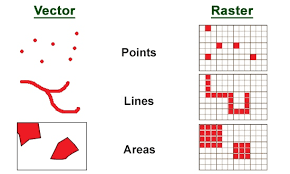
\includegraphics[width=0.70\textwidth]{figuras/dados-vetoriais-matriciais.png}
    \label{fig:dados-vetoriais-matriciais}
    \fonte{Imagem disponibilizada em \citeonline{Yusuf2016}.}
\end{figure}


\subsection{Sistemas de Referência Espacial}
\label{sec:sistemas-referencia}

Para que dados provenientes de diferentes fontes possam ser apresentados corretamente em uma mesma visualização cartográfica, é necessário estabelecer como suas coordenadas correspondem à superfície terrestre. Os sistemas de referência espacial definem os parâmetros utilizados para interpretar essas coordenadas, considerando aspectos como o sistema de coordenadas, o datum geodésico e, quando aplicável, a projeção cartográfica. Nos sistemas de coordenadas geográficas, as posições são expressas por latitude e longitude, geralmente em graus, enquanto os sistemas projetados utilizam coordenadas planas, frequentemente representadas em metros \cite{QGISCoordenadas2025}. A Figura \ref{fig:coordenadas-geograficas} ilustra a organização das coordenadas geográficas a partir dos paralelos e meridianos terrestres.

\begin{figure}[htb]
    \centering
    \caption{Representação das coordenadas geográficas de latitude e longitude}
    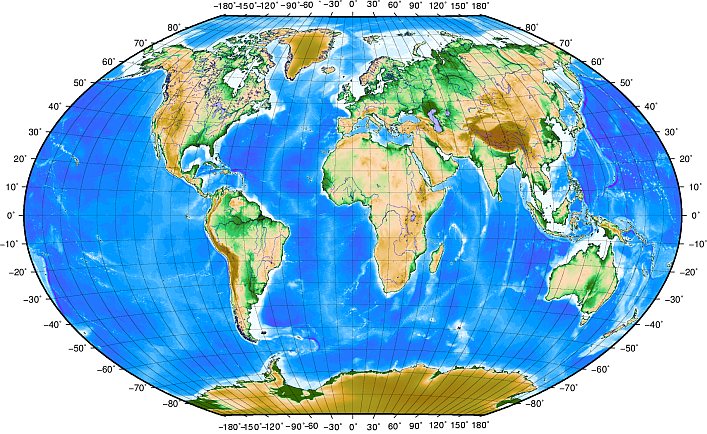
\includegraphics[width=0.70\textwidth]{figuras/coordenadas-geograficas.png}
    \label{fig:coordenadas-geograficas}
    \fonte{Imagem disponibilizada em \citeonline{QGISCoordenadas2025}.}
\end{figure}

Quando referências espaciais distintas não são consideradas adequadamente, camadas que representam uma mesma região podem apresentar deslocamentos ou incompatibilidades. Nesse contexto, a identificação dos sistemas de referência e, quando necessário, a transformação de coordenadas são fundamentais para garantir o alinhamento das informações. Em aplicações \gls{WebGIS}, bibliotecas cartográficas e servidores de mapas precisam interpretar corretamente essas referências, permitindo que dados provenientes de diferentes fontes sejam sobrepostos de maneira consistente.

\section{Sistemas de Informação Geográfica na Web}
\label{sec:webgis}

O avanço das tecnologias de Internet e dos navegadores possibilitou a disponibilização de funcionalidades geográficas diretamente na web, consolidando os Sistemas de Informação Geográfica na Web, conhecidos como WebGIS \cite{Silva2013}. \glsunset{WebGIS} Essas aplicações permitem acessar mapas e informações espaciais por meio de navegadores, sem exigir a instalação de programas especializados, oferecendo recursos como navegação cartográfica, alteração do nível de \textit{zoom}, ativação de camadas temáticas e consulta de informações geográficas.

As plataformas \gls{WebGIS} não substituem os programas tradicionais de geoprocessamento, que permanecem relevantes para atividades especializadas de edição, produção cartográfica e análise espacial. Sua principal contribuição está na ampliação do acesso e do compartilhamento das informações geográficas \cite{BastosCamboim2022}. Além disso, essas plataformas podem distribuir responsabilidades entre diferentes componentes, de modo que o armazenamento e a publicação dos dados sejam realizados no ambiente servidor, enquanto a visualização cartográfica e as interações com a interface ocorrem no navegador do usuário \cite{VinuezaMartinez2024}.

\subsection{WebGIS na Gestão Pública}
\label{sec:webgis-gestao-publica}

Na Administração Pública, as aplicações \gls{WebGIS} permitem reunir informações relacionadas à mobilidade urbana, à saúde, à educação, à infraestrutura e à organização territorial em uma interface cartográfica comum. Essa integração pode apoiar atividades de consulta e planejamento municipal, além de ampliar o acesso às informações geográficas por cidadãos, estudantes, pesquisadores e profissionais interessados no território \cite{Alcantara2015,Marotta2020}.

Entretanto, a utilidade dessas plataformas depende não apenas das funcionalidades disponibilizadas pela interface, mas também da qualidade e da atualização das bases geográficas, da consistência dos metadados e da disponibilidade dos serviços responsáveis pelo fornecimento das informações. Nesse contexto, a organização dos dados e a interoperabilidade entre os componentes constituem aspectos fundamentais para garantir a continuidade e a confiabilidade das informações apresentadas.



\section{Interoperabilidade e Padrões Geoespaciais}
\label{sec:interoperabilidade}

Uma plataforma geográfica pode integrar diferentes ferramentas responsáveis pelo armazenamento, processamento e visualização das informações espaciais, tornando necessários mecanismos de interoperabilidade entre seus componentes. Nesse contexto, o \textit{Open Geospatial Consortium} (OGC) desenvolve padrões que permitem a comunicação entre servidores, clientes cartográficos e ferramentas de geoprocessamento, reduzindo a dependência entre tecnologias específicas \cite{OGCWMS,OGCWFS,OGCWMTS}. \glsunset{OGC} Entre os principais serviços padronizados pelo \gls{OGC}, destacam-se o WMS, o WFS e o WMTS, que apresentam diferentes formas de disponibilização das informações geoespaciais.

\subsection{Web Map Service}
\label{sec:wms}

O \textit{Web Map Service} (WMS) estabelece uma interface padronizada para obtenção de representações cartográficas produzidas por servidores de mapas \cite{OGCWMS}. \glsunset{WMS} Por meio da operação \texttt{GetMap}, o cliente solicita camadas geográficas, informando parâmetros como extensão territorial, dimensões da imagem, sistema de referência e formato de saída, geralmente \texttt{PNG} ou \texttt{JPEG}. Entre esses parâmetros, a \texttt{BBOX} (\textit{Bounding Box}) delimita a área geográfica solicitada. Diferentemente de serviços que disponibilizam as feições completas, o \gls{WMS} fornece principalmente sua representação visual, permitindo que dados originalmente vetoriais sejam processados e apresentados como imagens cartográficas.

\subsection{Web Feature Service e GeoJSON}
\label{sec:wfs}

O \textit{Web Feature Service} (WFS) permite acessar diretamente feições geográficas e seus atributos, diferentemente do \gls{WMS}, que disponibiliza principalmente representações cartográficas \cite{OGCWFS}. \glsunset{WFS} Dessa forma, pontos, linhas e polígonos podem ser consultados e transferidos ao cliente para operações de seleção, filtragem e análise espacial. Entre os formatos utilizados para representar essas informações encontra-se o \texttt{GeoJSON}, padronizado pelo RFC 7946, que emprega a estrutura \gls{JSON} para organizar geometrias e atributos descritivos \cite{RFC7946}. Entretanto, o \texttt{GeoJSON} constitui um formato de dados, e não um serviço geoespacial, podendo ser utilizado independentemente ou como resposta de determinadas implementações de \gls{WFS}.

\subsection{Web Map Tile Service}
\label{sec:wmts}

O \textit{Web Map Tile Service} (WMTS) disponibiliza representações cartográficas organizadas em mosaicos de imagens, denominados \textit{tiles}, distribuídos em matrizes associadas a níveis de escala predefinidos \cite{OGCWMTS}. \glsunset{WMTS} Essa organização permite solicitar apenas os mosaicos necessários à área visualizada, favorecendo o armazenamento e o reaproveitamento das imagens por mecanismos de \textit{cache}. Diferentemente do \gls{WMS}, que permite solicitar representações para extensões geográficas arbitrárias, o \gls{WMTS} utiliza matrizes e níveis de escala padronizados, facilitando a reutilização dos mosaicos cartográficos.

A Tabela \ref{tab:comparativo-ogc} sintetiza as principais características dos serviços apresentados.

\begin{table}[!htbp]
    \captionsetup{width=15cm}
    \Caption{\label{tab:comparativo-ogc} Comparativo entre serviços geoespaciais}
    \IBGEtab{}{
        \begin{tabular}{p{3.0cm}p{3.6cm}p{3.6cm}p{3.6cm}}
            \toprule
            \textbf{Característica} & \textbf{WMS} & \textbf{WFS} & \textbf{WMTS} \\
            \midrule \midrule

            Conteúdo fornecido &
            Imagens cartográficas &
            Feições e atributos &
            Mosaicos de imagens \\
            \midrule

            Geometrias disponíveis &
            Não diretamente &
            Sim &
            Não diretamente \\
            \midrule

            Forma de consulta &
            Área geográfica e camadas &
            Feições e filtros &
            Matrizes e níveis de escala \\
            \midrule

            Processamento &
            Renderização no servidor &
            Processamento também no cliente &
            Mosaicos e mecanismos de cache \\
            \midrule

            Aplicações comuns &
            Camadas temáticas &
            Consulta de dados vetoriais &
            Mapas de base e mosaicos \\

            \bottomrule
        \end{tabular}
    }{
        \fonte{Elaborado pelo autor.}
    }
\end{table}

Embora esses padrões ofereçam diferentes formas de acesso às informações geográficas, o ``Sobral em Mapas'' utiliza principalmente o \gls{WMS} para consumir as camadas temáticas publicadas pelo GeoServer. O formato \texttt{GeoJSON}, por sua vez, é empregado na representação do limite territorial do município, sem a necessidade de utilização do \gls{WFS} na implementação desenvolvida.


\section{Arquitetura de Software em Aplicações Web}
\label{sec:arquitetura-software}

A arquitetura de software estabelece a organização dos principais componentes de um sistema, definindo suas responsabilidades e formas de comunicação \cite{Bass2021}. Essas decisões influenciam aspectos como manutenção, evolução, implantação e integração, sendo necessário considerar as características e os requisitos de cada aplicação na escolha da abordagem arquitetural.

\subsection{Arquitetura Monolítica e Arquitetura Desacoplada}
\label{sec:arquiteturas-web}

Na arquitetura monolítica, os diferentes módulos do sistema são reunidos em uma aplicação principal, geralmente desenvolvida e implantada como uma unidade. Essa abordagem pode simplificar a organização inicial de projetos menores, pois concentra funcionalidades e reduz a necessidade de comunicação entre serviços independentes. Entretanto, conforme a aplicação cresce, o aumento das dependências internas pode dificultar determinadas alterações e processos de implantação.

A arquitetura desacoplada, por sua vez, distribui responsabilidades entre componentes que se comunicam por interfaces bem definidas. Em aplicações web, essa separação ocorre frequentemente entre o \textit{front-end}, responsável pela interface e interação com o usuário, e o \textit{back-end}, que concentra regras de negócio, persistência e segurança. Em sistemas geoespaciais, essa organização pode incluir um servidor de mapas, responsável pela publicação das informações cartográficas.

A separação das responsabilidades pode favorecer a manutenção e a evolução dos componentes, desde que os contratos de comunicação sejam preservados. Por outro lado, exige maior atenção à configuração e à integração entre os serviços. A Tabela \ref{tab:comparativo-arquitetura} apresenta uma comparação entre as duas abordagens.

\begin{table}[htb]
    \captionsetup{width=15cm}
    \Caption{\label{tab:comparativo-arquitetura} Comparação entre arquitetura monolítica e desacoplada}
    \IBGEtab{}{
        \begin{tabular}{p{3.0cm}p{5.1cm}p{5.1cm}}
            \toprule
            \textbf{Característica} &
            \textbf{Monolítica} &
            \textbf{Desacoplada} \\
            \midrule \midrule

            Organização &
            Componentes reunidos em uma aplicação &
            Responsabilidades distribuídas entre componentes \\
            \midrule

            Implantação &
            Geralmente realizada como uma unidade &
            Pode ocorrer de forma independente \\
            \midrule

            Comunicação &
            Predominantemente interna &
            Realizada por interfaces e protocolos \\
            \midrule

            Manutenção &
            Alterações podem envolver diferentes módulos &
            Favorece a separação das modificações \\
            \midrule

            Infraestrutura &
            Pode apresentar menor complexidade inicial &
            Pode exigir maior configuração e integração \\

            \bottomrule
        \end{tabular}
    }{
        \fonte{Elaborado pelo autor.}
    }
\end{table}

\subsection{Single Page Application}
\label{sec:spa}

Uma \textit{Single Page Application} (SPA) é uma abordagem de desenvolvimento na qual a aplicação carrega inicialmente sua estrutura principal e atualiza dinamicamente partes da interface, sem exigir o recarregamento completo da página a cada interação. \glsunset{SPA} Esse comportamento permite construir interfaces interativas, nas quais diferentes componentes podem apresentar informações e responder às ações dos usuários de maneira integrada.

Em aplicações cartográficas, a utilização de uma \gls{SPA} permite manter o mapa, os painéis e as ferramentas ativos enquanto camadas e informações são atualizadas. Entretanto, essa abordagem não elimina a comunicação com o servidor, pois a aplicação continua realizando requisições para recuperar dados, autenticar usuários e executar operações relacionadas às regras de negócio.

\subsection{APIs e Arquitetura REST}
\label{sec:api-rest}

A comunicação entre componentes de uma arquitetura desacoplada pode ocorrer por meio de Interfaces de Programação de Aplicações (APIs), que estabelecem operações e contratos para a troca de informações entre sistemas. Em aplicações web, essa comunicação utiliza frequentemente o protocolo \gls{HTTP} e formatos estruturados, como \gls{JSON}, permitindo que diferentes tecnologias compartilhem dados por interfaces padronizadas.

O \textit{Representational State Transfer} (REST) é um estilo arquitetural para sistemas distribuídos apresentado por \citeonline{Fielding2000}. \glsunset{REST} Entre seus princípios destacam-se a separação entre cliente e servidor, a identificação de recursos e a comunicação sem a manutenção obrigatória de estado de sessão entre as requisições. Esses princípios orientam a organização de APIs voltadas à manipulação e à consulta de recursos.

Nas APIs baseadas em \gls{HTTP}, métodos como \texttt{GET}, \texttt{POST}, \texttt{PUT}, \texttt{PATCH} e \texttt{DELETE} são utilizados para representar diferentes operações. As respostas também empregam códigos de estado, sendo a família \texttt{2xx} associada geralmente ao sucesso da solicitação, \texttt{4xx} a problemas relacionados à requisição ou ao acesso, e \texttt{5xx} a falhas no processamento pelo servidor.


\section{Tecnologias de Desenvolvimento da Plataforma}
\label{sec:tecnologias}

O desenvolvimento de uma plataforma \gls{WebGIS} envolve tecnologias responsáveis pela interface cartográfica, pelo processamento das requisições, pelo armazenamento das informações administrativas e pela publicação dos dados geoespaciais. Esta seção apresenta as principais ferramentas relacionadas a essas responsabilidades.

\subsection{React, Leaflet e React-Leaflet}
\label{sec:frontend-tecnologias}

React é uma biblioteca JavaScript utilizada na construção de interfaces baseadas em componentes reutilizáveis \cite{ReactDocs}. Essa abordagem permite organizar funcionalidades e gerenciar estados da aplicação, como camadas selecionadas, painéis abertos e informações do usuário. Para a visualização cartográfica, Leaflet disponibiliza recursos de navegação, gerenciamento de camadas, representação de geometrias e integração com serviços geoespaciais, incluindo o \gls{WMS} \cite{LeafletDocs}. O React-Leaflet, por sua vez, integra esses recursos aos componentes React, permitindo controlar elementos do mapa por meio dos estados da aplicação \cite{ReactLeafletDocs}. Essa integração também pode ser ampliada com extensões destinadas a desenhos, medições e outras interações cartográficas.

\subsection{Laravel, Eloquent e Laravel Sanctum}
\label{sec:backend-tecnologias}

Laravel é um \textit{framework} PHP que oferece recursos para organização de aplicações web, incluindo rotas, validação, autenticação e acesso a bancos de dados \cite{LaravelDocs8}. Além de aplicações tradicionais, permite desenvolver APIs destinadas à comunicação com interfaces independentes, mantendo o processamento das regras de negócio no servidor.
O Eloquent é o mecanismo de Mapeamento Objeto-Relacional do Laravel, responsável por representar tabelas e relacionamentos do banco de dados por meio de modelos \cite{LaravelEloquent8}. Complementarmente, Laravel Sanctum fornece mecanismos de autenticação para aplicações e APIs, incluindo o uso de \textit{tokens} associados aos usuários \cite{LaravelSanctum8}. Em conjunto com as regras de autorização implementadas no servidor, esses recursos permitem controlar o acesso às funcionalidades administrativas.

\subsection{Banco de Dados MySQL}
\label{sec:mysql}

MySQL é um Sistema Gerenciador de Banco de Dados Relacional que organiza informações em tabelas relacionadas por chaves primárias e estrangeiras \cite{MySQL80}. Em uma plataforma \gls{WebGIS}, pode armazenar usuários, perfis, categorias, subcategorias e metadados das camadas, enquanto os dados geográficos podem permanecer em fontes externas especializadas. Essa separação distingue a persistência administrativa da publicação cartográfica.

\subsection{GeoServer}
\label{sec:geoserver}

GeoServer é um servidor de mapas de código aberto que permite publicar informações geoespaciais por meio de padrões interoperáveis, como \gls{WMS} e \gls{WFS} \cite{GeoServerDocs}. Sua utilização separa a disponibilização cartográfica das operações administrativas da aplicação, permitindo que a API gerencie usuários e metadados enquanto os serviços geoespaciais fornecem as camadas. Quando essa infraestrutura é externa, a integração depende da disponibilidade e da configuração dos recursos publicados.

A Tabela \ref{tab:responsabilidades-tecnologias} sintetiza as responsabilidades das principais tecnologias apresentadas.

\begin{table}[!htbp]
    \captionsetup{width=15cm}
    \Caption{\label{tab:responsabilidades-tecnologias} Principais tecnologias e responsabilidades em uma arquitetura WebGIS}
    \IBGEtab{}{
        \begin{tabular}{p{3.5cm}p{4.8cm}p{4.8cm}}
            \toprule
            \textbf{Tecnologia} &
            \textbf{Responsabilidade principal} &
            \textbf{Contexto de utilização} \\
            \midrule \midrule

            React &
            Construção da interface &
            Componentes e gerenciamento de estados \\
            \midrule

            Leaflet / React-Leaflet &
            Visualização cartográfica &
            Mapas, camadas e ferramentas de interação \\
            \midrule

            Laravel &
            Processamento da API &
            Regras de negócio, validação e autenticação \\
            \midrule

            MySQL &
            Persistência administrativa &
            Usuários, categorias e metadados \\
            \midrule

            GeoServer &
            Publicação geoespacial &
            Camadas e serviços OGC \\

            \bottomrule
        \end{tabular}
    }{
        \fonte{Elaborado pelo autor.}
    }
\end{table}

\section{Conteinerização e Computação em Nuvem}
\label{sec:infraestrutura}

Aplicações \textit{web} dependem de bibliotecas e configurações que podem variar entre os ambientes de desenvolvimento e produção, ocasionando incompatibilidades. Nesse contexto, a conteinerização permite padronizar ambientes ao reunir aplicações e dependências em contêineres isolados. Docker é uma plataforma utilizada para construir e executar esses ambientes, com instruções definidas em um arquivo \texttt{Dockerfile} \cite{DockerContainers}. Já o Docker Compose permite configurar a execução conjunta de serviços, incluindo redes, volumes e portas \cite{DockerCompose}.

Em arquiteturas desacopladas, os componentes podem ser hospedados em infraestruturas distintas. A computação em nuvem disponibiliza recursos computacionais por meio de provedores externos \cite{MellGrance2011}, permitindo distribuir a execução de interfaces, APIs e outros serviços. No ``Sobral em Mapas'', esses conceitos fundamentam a padronização do ambiente do \textit{back-end} e a implantação independente do \textit{front-end} e da API, conforme detalhado na Metodologia.

\section{Responsividade e Usabilidade em Aplicações WebGIS}
\label{sec:usabilidade}

Aplicações \textit{web} são acessadas por dispositivos com diferentes dimensões de tela e modalidades de interação, exigindo adaptações na interface. O desenvolvimento responsivo busca manter as funcionalidades acessíveis em computadores, tablets e dispositivos móveis. Nas plataformas \gls{WebGIS}, esse aspecto é especialmente relevante, pois o mapa precisa coexistir com menus, painéis e ferramentas de navegação, preservando condições adequadas de visualização e interação.

A organização da interface também está relacionada à usabilidade, definida pela ISO 9241-11 em termos de efetividade, eficiência e satisfação de usuários específicos em determinado contexto de uso \cite{ISO9241112018}. Em aplicações cartográficas, a clareza dos controles, a identificação das ferramentas e a organização das camadas podem favorecer a interação. Esses princípios orientam a estruturação da interface, sem pressupor uma avaliação formal de usabilidade.


\section{Trabalhos Relacionados}
\label{sec:trabalhos-relacionados}

O desenvolvimento de plataformas WebGIS tem sido abordado em diferentes pesquisas, especialmente no contexto da disponibilização de informações geoespaciais e da integração entre tecnologias cartográficas. Nesse sentido, \citeonline{Alcantara2015} apresentam a plataforma Geoinfo, desenvolvida no âmbito da Embrapa, utilizando a região do Matopiba como exemplo de aplicação. A solução contempla a organização e a disseminação de dados vetoriais e matriciais, evidenciando o potencial das plataformas WebGIS para a categorização e a integração de informações geoespaciais.

Em uma abordagem voltada à gestão territorial municipal, \citeonline{Marotta2020} descrevem o desenvolvimento do WebGENTE, uma plataforma WebGIS destinada à visualização de informações cadastrais do município de Bom Despacho. A solução utiliza Leaflet e GeoServer, disponibilizando recursos de consulta, pesquisa por atributos e controle de acesso conforme os níveis de usuário. O estudo demonstra a aplicação de tecnologias abertas na construção de interfaces cartográficas voltadas à disponibilização de dados municipais, apresentando semelhanças com a proposta do ``Sobral em Mapas''.

Sob uma perspectiva relacionada à publicação cartográfica, \citeonline{BastosCamboim2022} comparam diferentes abordagens para disponibilização de mapas topográficos na web, considerando os serviços WMS, arquivos GeoJSON e mosaicos vetoriais (\textit{Vector Tiles}). A pesquisa analisa aspectos como desempenho, volume de dados transferidos, interatividade e qualidade gráfica, evidenciando diferenças entre as alternativas avaliadas. Essas contribuições são relevantes para compreender as possibilidades de integração geoespacial e contextualizar a utilização do WMS na plataforma desenvolvida.

Embora compartilhem características relacionadas à visualização e à disponibilização de informações geográficas, os trabalhos apresentam objetivos e contextos de aplicação distintos. O ``Sobral em Mapas'' concentra-se no desenvolvimento de uma plataforma municipal que integra ferramentas de consulta cartográfica, gerenciamento administrativo de usuários e metadados das camadas, além do consumo de serviços WMS disponibilizados por uma infraestrutura geoespacial externa. Dessa forma, a proposta enfatiza a aplicação de princípios de Engenharia de Software na organização de uma arquitetura desacoplada, associando a interface pública aos mecanismos administrativos necessários à disponibilização das informações.

\section{Considerações do Capítulo}
\label{sec:consideracoes-fundamentacao}

Os conceitos apresentados neste capítulo fundamentam a estrutura e o funcionamento do ``Sobral em Mapas''. Os Sistemas de Informação Geográfica e as plataformas \gls{WebGIS} explicam a representação e a disponibilização das informações espaciais, enquanto os padrões do \gls{OGC}, especialmente o \gls{WMS}, fundamentam a comunicação com serviços geoespaciais. Além disso, a arquitetura desacoplada, as \gls{SPA} e as APIs orientam a distribuição de responsabilidades entre os componentes da aplicação.

As tecnologias React, Leaflet, React-Leaflet, Laravel, MySQL e GeoServer sustentam a construção da interface, o gerenciamento administrativo e a disponibilização cartográfica. A conteinerização e a computação em nuvem complementam a organização dos ambientes de execução, enquanto a responsividade e a usabilidade orientam a estruturação da interface. Com base nesses fundamentos e na análise dos trabalhos relacionados, o capítulo seguinte apresenta a Metodologia, abrangendo os requisitos, a arquitetura da solução, o desenvolvimento e os procedimentos de verificação da plataforma.

    \chapter{Metodologia}
\label{cap:metodologia}

Este capítulo apresenta os procedimentos metodológicos e as principais decisões adotadas no desenvolvimento da plataforma ``Sobral em Mapas''. São descritos a caracterização da pesquisa, o levantamento dos requisitos, a arquitetura da solução, a modelagem dos dados, o desenvolvimento do back-end e do front-end, a integração com o GeoServer, a configuração do ambiente de execução e os procedimentos de verificação das funcionalidades. A solução foi desenvolvida segundo uma arquitetura desacoplada, com separação entre a interface, as regras de negócio, a persistência dos dados administrativos e os serviços geoespaciais.

\section{Caracterização da Pesquisa}
\label{sec:caracterizacao-pesquisa}

Este trabalho caracteriza-se como uma pesquisa de natureza aplicada e predominantemente descritiva \cite{ProdanovFreitas2013}, direcionada ao desenvolvimento de uma solução computacional para organização, integração e disponibilização de informações geográficas relacionadas ao município de Sobral. O trabalho também possui caráter tecnológico, pois envolve a construção e a integração dos componentes necessários ao funcionamento da plataforma WebGIS.

O desenvolvimento foi conduzido de forma incremental. Inicialmente, foram identificadas as necessidades da plataforma e definidos seus requisitos e sua arquitetura. Em seguida, foram desenvolvidos o back-end, o front-end e os recursos cartográficos, posteriormente integrados ao banco de dados, aos serviços geoespaciais e ao ambiente de execução. Durante esse processo, ciclos de implementação, verificação e refinamento permitiram realizar ajustes progressivos nas funcionalidades e nos fluxos de comunicação.

A abordagem metodológica adotada pode ser sintetizada nas seguintes etapas:

\begin{alineascomponto}

    \item levantamento e especificação dos requisitos da plataforma;

    \item definição da arquitetura e modelagem dos dados administrativos;

    \item desenvolvimento da API, dos mecanismos de autenticação e do gerenciamento dos dados;

    \item desenvolvimento da interface web e dos recursos cartográficos;

    \item integração com os serviços geoespaciais disponibilizados pelo GeoServer;

    \item configuração do ambiente de execução e conteinerização do back-end;

    \item verificação das funcionalidades e dos fluxos integrados da plataforma.

\end{alineascomponto}

As etapas não foram executadas de maneira estritamente linear, uma vez que requisitos e componentes foram revisados durante a implementação e a integração. Esse processo possibilitou o refinamento progressivo da solução até a versão apresentada neste trabalho.

\section{Visão Geral do Sistema}
\label{sec:visao-geral}

A aplicação ``Sobral em Mapas'' constitui-se como uma plataforma WebGIS desenvolvida para o município de Sobral, com a finalidade de disponibilizar uma interface interativa para a visualização e a organização de informações geográficas de interesse público e administrativo. A solução foi concebida segundo uma arquitetura desacoplada, distribuindo suas principais responsabilidades entre componentes independentes que atuam de maneira integrada.

De forma geral, a plataforma pode ser compreendida a partir de quatro componentes principais:

\begin{alineascomponto}

    \item \textbf{Cliente cartográfico (front-end):} desenvolvido como uma Single Page Application (SPA) em React, é responsável pela interface com o usuário, pela adaptação dos componentes a diferentes dispositivos e pela visualização cartográfica utilizando Leaflet e React-Leaflet;

    \item \textbf{Servidor de aplicação (back-end):} implementado com o framework PHP Laravel, disponibiliza uma API responsável pelas regras de negócio, autenticação, autorização, gerenciamento dos dados administrativos e intermediação das requisições aos serviços geoespaciais;

    \item \textbf{Serviço de dados geoespaciais:} representado pelo GeoServer, é responsável pela publicação e disponibilização das camadas cartográficas por meio de serviços interoperáveis, especialmente o Web Map Service (WMS);

    \item \textbf{Camada de persistência:} composta pelo banco de dados MySQL, armazena as informações administrativas da aplicação, incluindo usuários, perfis, categorias, subcategorias, camadas e referências aos serviços WMS.

\end{alineascomponto}

Essa organização estabelece uma separação entre a interface, o processamento das regras de negócio, o armazenamento das informações administrativas e a disponibilização dos dados geoespaciais. Dessa forma, busca-se reduzir o acoplamento entre os componentes e favorecer a manutenção, a evolução das funcionalidades e a integração com serviços externos.

A Figura \ref{fig:arquitetura-geral} apresenta a visão geral dos componentes da plataforma e suas principais relações de comunicação.

\begin{figure}[htb]
    \centering
    \caption{\label{fig:arquitetura-geral} Visão geral dos componentes da plataforma Sobral em Mapas}
    \includegraphics[width=\textwidth]{figuras/arquitetura-geral.pdf}
    \fonte{Elaborado pelo autor.}
\end{figure}

\section{Levantamento e Especificação de Requisitos}
\label{sec:requisitos}

A definição dos requisitos da plataforma foi realizada a partir dos objetivos estabelecidos para o ``Sobral em Mapas'', considerando as funcionalidades necessárias à consulta das informações geográficas, à interação com a interface cartográfica e ao gerenciamento administrativo dos elementos utilizados pelo sistema. Os requisitos foram consolidados ao longo do processo de desenvolvimento e refinados à medida que os diferentes componentes da aplicação eram implementados e integrados, permitindo adequações decorrentes das características da arquitetura adotada e das necessidades identificadas durante a construção da interface.

Para fins de organização, os requisitos foram classificados em funcionais e não funcionais. Os requisitos funcionais descrevem os comportamentos e serviços disponibilizados pela plataforma aos seus usuários, enquanto os requisitos não funcionais estabelecem características e restrições relacionadas à arquitetura, segurança, interoperabilidade, manutenção, responsividade e execução do sistema.


\subsection{Perfis de Interação com o Sistema}
\label{sec:perfis-usuario}

A plataforma disponibiliza funcionalidades públicas e administrativas, tornando necessário distinguir os diferentes níveis de interação e acesso ao sistema. As funcionalidades cartográficas de consulta podem ser utilizadas sem autenticação, enquanto determinadas operações dependem da existência de um usuário autenticado e do perfil associado à sua conta. Para fins de especificação dos requisitos, foram considerados três perfis principais:

\begin{alineascomponto}

    \item \textbf{Visitante:} corresponde ao perfil destinado aos usuários que não possuem privilégios administrativos. As funcionalidades públicas da plataforma, como a visualização do mapa, a consulta das camadas e a utilização das ferramentas cartográficas, permanecem acessíveis independentemente de autenticação, enquanto o cadastro permite identificar o usuário sem conceder acesso às operações administrativas;

    \item \textbf{Administrador:} corresponde ao usuário autenticado com permissão para acessar as funcionalidades administrativas relacionadas ao gerenciamento dos conteúdos da plataforma, incluindo categorias, subcategorias, camadas e serviços WMS;

    \item \textbf{Superadministrador:} representa o perfil com maior nível de acesso à plataforma, reunindo as funcionalidades administrativas e as operações relacionadas ao gerenciamento de usuários, à atribuição dos perfis de acesso e ao controle das condições de utilização das áreas protegidas do sistema.

\end{alineascomponto}

A distinção entre esses perfis permite separar as funcionalidades destinadas à consulta pública das operações capazes de modificar informações administrativas da aplicação. O controle das operações protegidas é realizado no lado servidor, evitando que as restrições de acesso dependam exclusivamente dos elementos apresentados pela interface.



\subsection{Requisitos Funcionais}
\label{sec:requisitos-funcionais}

Os requisitos funcionais descrevem as principais operações disponibilizadas pela plataforma. Para evitar a fragmentação de funcionalidades pertencentes a um mesmo contexto de uso, recursos relacionados foram agrupados em requisitos mais abrangentes, contemplando tanto as ferramentas de consulta e interação cartográfica quanto as operações administrativas. A Tabela \ref{tab:requisitos-funcionais} apresenta os requisitos considerados durante o desenvolvimento.

\begin{table}[htb]
    \captionsetup{width=15cm}
    \Caption{\label{tab:requisitos-funcionais} Requisitos funcionais da plataforma Sobral em Mapas}
    \IBGEtab{}{
        \begin{tabular}{p{1.6cm}p{12.8cm}}
            \toprule
            \textbf{Código} & \textbf{Descrição} \\
            \midrule \midrule

            RF01 &
            Disponibilizar uma interface cartográfica interativa para visualização das informações geográficas do município de Sobral, apresentando as camadas temáticas organizadas por categorias e subcategorias. \\
            \midrule

            RF02 &
            Permitir pesquisar, ativar e desativar camadas geográficas, bem como consultar as legendas associadas à sua representação cartográfica. \\
            \midrule

            RF03 &
            Disponibilizar mecanismo de pesquisa de localização, permitindo localizar endereços ou pontos de interesse e reposicionar a visualização do mapa. \\
            \midrule

            RF04 &
            Disponibilizar ferramentas de medição de distâncias e áreas por meio de interações diretamente sobre o mapa. \\
            \midrule

            RF05 &
            Disponibilizar recursos auxiliares de interação cartográfica, incluindo favoritos, limpeza da visualização, modo de tela cheia e impressão ou exportação do mapa. \\
            \midrule

            RF06 &
            Disponibilizar um formulário de contato para o envio de mensagens pelos usuários da plataforma. \\
            \midrule

            RF07 &
            Permitir o cadastro e a autenticação de usuários, controlando o acesso às funcionalidades restritas conforme o perfil e a situação de aprovação da conta. \\
            \midrule

            RF08 &
            Permitir o gerenciamento dos usuários da aplicação, incluindo informações cadastrais, perfis de acesso e situação de aprovação. \\
            \midrule

            RF09 &
            Permitir o gerenciamento das categorias e subcategorias utilizadas na organização temática das camadas geográficas. \\
            \midrule

            RF10 &
            Permitir o gerenciamento dos cadastros e metadados das camadas geográficas, incluindo sua identificação, classificação e referências aos serviços WMS utilizados pela plataforma. \\

            \bottomrule
        \end{tabular}
    }{
        \Fonte{Elaborado pelo autor.}
    }
\end{table}

Os requisitos RF01 a RF06 estão associados principalmente às funcionalidades públicas da plataforma, enquanto o RF07 contempla o cadastro, a autenticação e o controle de acesso dos usuários. Por sua vez, os requisitos RF08 a RF10 abrangem o gerenciamento das informações administrativas necessárias ao funcionamento do sistema. Essa organização evidencia a relação entre a interface pública e o ambiente administrativo, uma vez que categorias, subcategorias, camadas e referências aos serviços WMS são gerenciadas pela aplicação e utilizadas na composição dos conteúdos cartográficos disponibilizados aos usuários.


\subsection{Requisitos Não Funcionais}
\label{sec:requisitos-nao-funcionais}

Além das funcionalidades disponibilizadas, foram definidos requisitos não funcionais relacionados à organização arquitetural, à segurança, à interoperabilidade, à responsividade e às condições de execução da plataforma. Esses requisitos orientaram as decisões técnicas e a estruturação dos componentes utilizados durante o desenvolvimento. A Tabela \ref{tab:requisitos-nao-funcionais} apresenta os principais requisitos não funcionais considerados.

\begin{table}[htb]
    \captionsetup{width=15cm}
    \Caption{\label{tab:requisitos-nao-funcionais} Requisitos não funcionais da plataforma Sobral em Mapas}
    \IBGEtab{}{
        \begin{tabular}{p{1.6cm}p{12.8cm}}
            \toprule
            \textbf{Código} & \textbf{Descrição} \\
            \midrule \midrule

            RNF01 &
            A interface deve apresentar comportamento responsivo, adaptando seus principais componentes a computadores, tablets e dispositivos móveis. \\
            \midrule

            RNF02 &
            A arquitetura deve manter separadas as responsabilidades do cliente web, do servidor de aplicação, da persistência dos dados administrativos e dos serviços geoespaciais. \\
            \midrule

            RNF03 &
            A plataforma deve utilizar padrões interoperáveis para o consumo de informações geoespaciais, especialmente o serviço WMS disponibilizado pelo GeoServer. \\
            \midrule

            RNF04 &
            As funcionalidades administrativas devem ser protegidas por mecanismos de autenticação e autorização implementados no lado servidor. \\
            \midrule

            RNF05 &
            Os dados recebidos pela API devem ser validados antes da execução das operações de persistência. \\
            \midrule

            RNF06 &
            O front-end deve ser organizado em componentes reutilizáveis, favorecendo a manutenção e a evolução da interface. \\
            \midrule

            RNF07 &
            A comunicação entre o front-end e o back-end deve utilizar HTTP/HTTPS, empregando JSON para os dados administrativos e respostas compatíveis com as requisições cartográficas intermediadas pela API. \\
            \midrule

            RNF08 &
            O ambiente de execução do back-end deve possuir configuração reproduzível por meio de conteinerização com Docker. \\
            \midrule

            RNF09 &
            As funcionalidades públicas devem ser acessíveis diretamente por navegador web, sem exigir a instalação de softwares especializados de geoprocessamento. \\
            \midrule

            RNF10 &
            As configurações específicas dos ambientes de desenvolvimento e produção devem ser gerenciadas por variáveis de ambiente, evitando alterações diretas no código-fonte durante a implantação. \\

            \bottomrule
        \end{tabular}
    }{
        \Fonte{Elaborado pelo autor.}
    }
\end{table}

Os requisitos não funcionais orientaram as decisões arquiteturais e tecnológicas adotadas durante o desenvolvimento. A separação entre os componentes da plataforma relaciona-se ao RNF02, enquanto a integração com o GeoServer por meio do WMS atende ao requisito de interoperabilidade definido no RNF03. Os mecanismos de autenticação, autorização e validação das requisições estão associados aos requisitos RNF04 e RNF05. Além disso, a componentização da interface, a conteinerização do back-end e a configuração dos ambientes contribuem para atender aos requisitos RNF06, RNF08 e RNF10. A correspondência entre os requisitos estabelecidos e os resultados observados durante a verificação da plataforma será retomada no capítulo de Resultados e Discussão.


\section{Arquitetura da Solução}
\label{sec:arquitetura-solucao}

A arquitetura do ``Sobral em Mapas'' foi organizada de maneira desacoplada, estabelecendo interfaces de comunicação entre o cliente React, a API Laravel, o banco de dados MySQL e os serviços geoespaciais disponibilizados pelo GeoServer. Essa abordagem permite que cada componente desempenhe suas funções específicas, favorecendo a manutenção e a evolução da plataforma, desde que os contratos de comunicação sejam preservados.

A comunicação entre o front-end e o back-end ocorre por meio de requisições HTTP/HTTPS, utilizando principalmente representações JSON nas operações administrativas. O Laravel centraliza o processamento dessas operações e o acesso ao MySQL, além de intermediar as requisições WMS destinadas ao GeoServer. Dessa forma, o gerenciamento dos dados administrativos e a disponibilização das camadas cartográficas seguem fluxos distintos, embora integrados, preservando a separação de responsabilidades entre os componentes.

\subsection{Fluxo de Comunicação entre os Componentes}
\label{sec:fluxo-comunicacao}

No carregamento da aplicação, o cliente solicita à API as informações necessárias à composição da interface, incluindo categorias, subcategorias e camadas. O Laravel consulta o MySQL e retorna esses registros ao front-end, permitindo construir dinamicamente os elementos apresentados ao usuário a partir das informações mantidas no ambiente administrativo.

Quando uma camada é ativada, seus metadados permitem identificar o recurso geoespacial correspondente. O cliente realiza uma solicitação ao endpoint de proxy WMS do Laravel, que encaminha a requisição ao GeoServer e devolve ao navegador a representação cartográfica utilizada pelo Leaflet. Diferentemente das operações administrativas, esse fluxo envolve principalmente imagens cartográficas geradas pelo servidor de mapas.

Nas operações administrativas, a comunicação entre cliente, API e banco de dados inclui mecanismos de autenticação, autorização e validação. Somente após essas verificações o servidor executa as alterações necessárias e retorna o resultado ao cliente, mantendo o controle das operações protegidas no back-end.

A Figura \ref{fig:fluxo-comunicacao} apresenta o fluxo de disponibilização de uma camada cartográfica, destacando a comunicação entre o cliente, a API Laravel e o GeoServer.

\begin{figure}[htb]
    \centering
    \caption{\label{fig:fluxo-comunicacao} Fluxo de comunicação para disponibilização de uma camada cartográfica}
    \includegraphics[width=0.45\textwidth]{figuras/fluxo-comunicacao.pdf}
    \fonte{Elaborado pelo autor.}
\end{figure}


\section{Modelagem dos Dados}
\label{sec:modelagem-dados}

A modelagem dos dados da plataforma foi definida a partir das necessidades administrativas identificadas durante o levantamento de requisitos e da arquitetura adotada para o sistema. Como as informações administrativas e os dados geoespaciais possuem responsabilidades distintas, o banco de dados MySQL é utilizado para armazenar os registros necessários ao gerenciamento da aplicação, enquanto os recursos geográficos são disponibilizados por meio dos serviços geoespaciais integrados à plataforma. Dessa forma, o banco administrativo concentra informações relacionadas aos usuários, aos perfis de acesso, à organização temática das camadas e às referências necessárias para identificação dos serviços WMS, sem assumir diretamente o armazenamento ou o processamento das geometrias apresentadas no mapa.

As principais entidades consideradas nessa estrutura são \texttt{User}, \texttt{Profile}, \texttt{Category}, \texttt{Subcategory}, \texttt{Layer} e \texttt{WmsLink}. Seus relacionamentos representam tanto o controle de acesso quanto a organização hierárquica e a associação das camadas aos serviços geoespaciais utilizados pela aplicação. A Figura \ref{fig:modelo-entidade-relacionamento} apresenta, de forma simplificada, o modelo entidade-relacionamento das principais entidades do banco de dados administrativo.

\begin{figure}[htb]
    \centering
    \caption{\label{fig:modelo-entidade-relacionamento} Modelo entidade-relacionamento das principais entidades da plataforma Sobral em Mapas}
    \includegraphics[width=0.90\textwidth]{figuras/modelo-entidade-relacionamento.pdf}
    \fonte{Elaborado pelo autor.}
\end{figure}


\subsection{Principais Entidades}
\label{sec:principais-entidades}

A entidade \texttt{User} representa os usuários cadastrados e reúne as informações necessárias à identificação, autenticação, perfil de acesso e situação de aprovação, enquanto \texttt{Profile} define os diferentes níveis de acesso da plataforma. As entidades \texttt{Category} e \texttt{Subcategory} organizam tematicamente as camadas, estabelecendo uma estrutura hierárquica e permitindo o controle de ativação desses agrupamentos.

A entidade \texttt{Layer} representa as camadas cadastradas e concentra os principais metadados necessários à sua identificação e utilização, como nome, identificador técnico, sistema de referência, tipo de serviço, ordem de exibição, situação de publicação e referências à subcategoria e ao serviço WMS. Por sua vez, \texttt{WmsLink} armazena o nome, o endereço e a versão dos serviços WMS utilizados pela aplicação. Dessa forma, os registros administrativos mantêm as informações necessárias à associação das camadas aos recursos geoespaciais, sem armazenar diretamente as feições exibidas no mapa.

A Tabela \ref{tab:entidades-principais} sintetiza as responsabilidades das principais entidades utilizadas na modelagem.

\begin{table}[htb]
    \captionsetup{width=15cm}
    \Caption{\label{tab:entidades-principais} Principais entidades da plataforma Sobral em Mapas}
    \IBGEtab{}{
        \begin{tabular}{p{3.2cm}p{5cm}p{6.2cm}}
            \toprule
            \textbf{Entidade} &
            \textbf{Responsabilidade} &
            \textbf{Informações associadas} \\
            \midrule \midrule

            \texttt{User} &
            Representar os usuários cadastrados na aplicação &
            Identificação, autenticação, perfil de acesso e situação de aprovação \\
            \midrule

            \texttt{Profile} &
            Definir os perfis de acesso utilizados pela plataforma &
            Identificação e classificação do perfil de acesso \\
            \midrule

            \texttt{Category} &
            Organizar as informações em grupos temáticos de nível superior &
            Identificação e situação de ativação \\
            \midrule

            \texttt{Subcategory} &
            Subdividir as categorias e organizar as camadas temáticas &
            Identificação, situação de ativação e referência à categoria \\
            \midrule

            \texttt{Layer} &
            Representar as camadas cadastradas na plataforma &
            Identificação, metadados cartográficos, organização, visibilidade e referências à subcategoria e ao serviço WMS \\
            \midrule

            \texttt{WmsLink} &
            Representar os serviços WMS cadastrados na aplicação &
            Nome, endereço do serviço e versão utilizada \\

            \bottomrule
        \end{tabular}
    }{
        \Fonte{Elaborado pelo autor.}
    }
\end{table}


\subsection{Relacionamentos entre as Entidades}
\label{sec:relacionamentos-entidades}

Os relacionamentos estabelecidos entre as entidades refletem o controle de acesso, a organização temática e a associação das camadas aos serviços geoespaciais. Cada registro de \texttt{User} está associado a um \texttt{Profile}, enquanto um mesmo perfil pode estar relacionado a diferentes usuários, estabelecendo uma relação de um para muitos. De maneira semelhante, uma \texttt{Category} pode reunir diversas \texttt{Subcategory}, enquanto cada subcategoria pertence a uma única categoria. Por sua vez, uma \texttt{Subcategory} pode agrupar diversas \texttt{Layer}, permitindo organizar hierarquicamente as informações cartográficas apresentadas pela plataforma.

A entidade \texttt{Layer} também pode manter uma referência a um registro de \texttt{WmsLink}, possibilitando que várias camadas utilizem um mesmo serviço WMS. Dessa forma, as informações referentes ao endereço e à versão do serviço permanecem centralizadas, enquanto cada camada mantém apenas a associação necessária à fonte geoespacial correspondente. Essa organização possibilita que categorias, subcategorias, camadas e serviços WMS sejam administrados de forma independente, preservando seus relacionamentos. Consequentemente, o front-end pode obter essas informações por meio da API e construir dinamicamente os agrupamentos e recursos apresentados ao usuário sem exigir alterações diretas na estrutura da interface.


\subsection{Separação entre Dados Administrativos e Dados Geoespaciais}
\label{sec:separacao-dados}

A separação entre dados administrativos e dados geoespaciais constitui uma das decisões centrais da modelagem adotada. O MySQL permanece responsável pelas informações necessárias à gestão da plataforma, incluindo usuários, perfis, organização temática, registros de camadas e referências aos serviços WMS, enquanto os dados utilizados para a representação cartográfica permanecem sob responsabilidade da infraestrutura geoespacial. Assim, um registro de \texttt{Layer} armazenado pela aplicação não corresponde ao conjunto de feições geográficas exibidas no mapa, funcionando principalmente como uma representação administrativa que reúne os metadados necessários à identificação e ao consumo do recurso correspondente.

Essa abordagem mantém separadas as responsabilidades dos componentes, pois o Laravel gerencia o cadastro, a classificação, os estados de ativação e os metadados relacionados às camadas, enquanto o GeoServer permanece responsável pela publicação e pela disponibilização das informações espaciais. Desse modo, alterações na organização administrativa da plataforma podem ser realizadas sem interferir diretamente nas fontes geográficas e, simultaneamente, a estrutura mantida no MySQL fornece ao front-end as informações necessárias para organizar, localizar e disponibilizar as camadas cartográficas ao usuário.


\section{Desenvolvimento do Back-end}
\label{sec:desenvolvimento-backend}

O back-end do ``Sobral em Mapas'' foi desenvolvido com Laravel e estruturado como uma API responsável pela comunicação entre a interface em React, o banco de dados MySQL e os serviços geoespaciais utilizados pela plataforma. Essa camada concentra o processamento das requisições, as regras de negócio, o acesso aos dados e os mecanismos de autenticação e autorização necessários ao funcionamento das áreas pública e administrativa.


\subsection{Estrutura e Preparação do Banco de Dados}
\label{sec:migrations-seeders}

A estrutura do banco de dados administrativo foi construída e modificada por meio das \textit{migrations} do Laravel. Esse mecanismo permite representar a criação e a alteração das tabelas como arquivos versionados, facilitando a reprodução da estrutura em diferentes ambientes. As migrations também foram utilizadas para definir chaves estrangeiras, restrições e relacionamentos necessários à integridade dos dados.

Inicialmente, foram criadas as tabelas relacionadas às categorias, subcategorias e camadas. Posteriormente, novas migrations ampliaram o esquema com os serviços WMS, seus relacionamentos com as camadas, os atributos de publicação e ativação, além das tabelas de usuários e perfis de acesso e do campo utilizado para representar a situação de aprovação dos cadastros. A preparação inicial dos dados utiliza os \textit{seeders} do Laravel. O \texttt{DatabaseSeeder} coordena a inserção de registros como perfis de acesso, usuários, categorias, subcategorias e camadas. Dessa forma, migrations e seeders atuam de maneira complementar: as primeiras definem e evoluem a estrutura do banco, enquanto os segundos fornecem os dados iniciais da aplicação.


\subsection{Organização da API}
\label{sec:organizacao-api}

A organização do servidor utiliza os recursos do Laravel para definição de rotas, controladores, modelos e middlewares. As rotas são declaradas principalmente no arquivo \texttt{routes/api.php}, que associa cada endpoint à operação correspondente e define, quando necessário, mecanismos de autenticação, verificação de perfil e limitação de requisições.

Embora o Laravel forneça uma estrutura relacionada ao padrão Model-View-Controller (MVC), no ``Sobral em Mapas'' ele é utilizado principalmente como servidor de API, uma vez que a camada visual é implementada em React. Os controladores processam as requisições, enquanto os modelos representam os registros persistidos no banco. Em algumas funcionalidades, também são utilizados serviços, repositórios e adaptadores para acesso aos dados e integração com recursos externos.

Essa organização mantém o back-end estruturado de forma modular, ainda que determinadas operações sejam realizadas diretamente pelos controladores em conjunto com os modelos Eloquent. De forma geral, a requisição é associada a uma rota, passa pelos mecanismos intermediários necessários e é encaminhada ao controlador responsável. O resultado é então devolvido ao cliente por meio de uma resposta HTTP, predominantemente em formato JSON, acompanhada do código de estado correspondente.

\subsection{Modelos e Persistência com Eloquent}
\label{sec:eloquent-persistencia}

O acesso ao banco de dados MySQL é realizado principalmente por meio do Eloquent, mecanismo de mapeamento objeto-relacional disponibilizado pelo Laravel. Com essa abordagem, as tabelas utilizadas pela aplicação são representadas por modelos e podem ser manipuladas por meio de métodos orientados a objetos, reduzindo a necessidade de utilização direta de instruções SQL nas operações usuais de consulta, inserção, atualização e exclusão.

Entre os principais modelos utilizados pela plataforma encontram-se aqueles relacionados aos usuários, perfis de acesso, categorias, subcategorias, camadas e serviços WMS. Os relacionamentos definidos no banco também são representados no Eloquent, permitindo, por exemplo, recuperar um usuário juntamente com seu perfil, obter as subcategorias associadas a uma categoria ou consultar uma camada em conjunto com sua classificação temática e sua referência ao serviço WMS. Esse mecanismo contribui para a construção das estruturas de dados posteriormente devolvidas ao front-end.

Um exemplo desse uso ocorre no carregamento da interface cartográfica, no qual a API consulta as camadas disponíveis juntamente com suas informações de organização e disponibiliza os resultados ao cliente. A mesma estrutura é utilizada no ambiente administrativo para criação, edição, ativação, desativação e remoção dos registros, mantendo o acesso ao banco concentrado no servidor e permitindo que as regras de validação e autorização sejam executadas antes da persistência das alterações.


\subsection{Autenticação e Controle de Acesso}
\label{sec:autenticacao-controle-acesso}

A autenticação dos usuários foi implementada utilizando os recursos do Laravel em conjunto com o Laravel Sanctum. Durante o processo de login, as credenciais fornecidas pela interface são encaminhadas à API e verificadas pelo servidor; quando as condições necessárias são atendidas, é gerado um token associado ao usuário autenticado. Esse token passa a acompanhar as requisições destinadas às rotas protegidas, permitindo que o servidor identifique o responsável pela operação sem exigir o reenvio das credenciais originais.

O controle de acesso complementa esse processo ao considerar o perfil associado ao usuário e a situação de aprovação do cadastro. A plataforma diferencia os usuários de acordo com níveis de permissão, permitindo restringir o acesso às funcionalidades administrativas conforme as responsabilidades atribuídas a cada perfil. Os usuários cadastrados pela interface pública permanecem inicialmente em situação pendente de aprovação, evitando que o próprio processo de cadastro resulte na atribuição automática de privilégios administrativos.

As rotas protegidas utilizam middlewares para verificar a presença de uma autenticação válida e, quando necessário, o perfil autorizado para determinada operação. Dessa maneira, as verificações de acesso são executadas antes que a requisição alcance a funcionalidade responsável pelo processamento. A API também disponibiliza operações destinadas à identificação do usuário autenticado e à revogação do token de autenticação.


\subsection{Validação e Tratamento das Requisições}
\label{sec:validacao-requisicoes}

Os dados recebidos pela API são submetidos às regras de validação disponibilizadas pelo Laravel antes que as operações de persistência sejam executadas. Essas verificações abrangem aspectos como o preenchimento dos campos obrigatórios, a validade dos endereços de e-mail, os requisitos mínimos definidos para senhas, a unicidade de determinados valores e a existência dos registros referenciados nos relacionamentos entre as entidades. Quando alguma das condições estabelecidas não é atendida, a operação é interrompida e o servidor devolve uma resposta indicando os problemas encontrados. Essa validação realizada no back-end complementa as verificações existentes na interface e impede que a consistência dos dados dependa exclusivamente do cliente.

As respostas também utilizam códigos de estado HTTP para diferenciar situações de sucesso de ocorrências relacionadas a dados inválidos, credenciais incorretas, ausência de autenticação, falta de autorização ou inexistência do recurso solicitado. Nas funcionalidades administrativas, essas verificações atuam em conjunto com os mecanismos de autenticação e autorização. Dessa forma, mesmo uma requisição que apresente dados estruturalmente válidos somente pode resultar em alteração das informações persistidas quando estiver associada a um usuário autenticado e devidamente autorizado para a operação solicitada.


\subsection{Principais Endpoints da API}
\label{sec:endpoints-api}

A comunicação entre o cliente e o servidor ocorre por meio dos endpoints disponibilizados pela API, que definem as operações necessárias ao funcionamento da interface pública e do ambiente administrativo. Além dos recursos de autenticação e cadastro, a API disponibiliza operações relacionadas ao carregamento das informações cartográficas, ao gerenciamento dos registros administrativos e à intermediação das requisições destinadas aos serviços WMS. A Tabela \ref{tab:principais-endpoints} apresenta alguns dos endpoints mais representativos da implementação.

\begin{table}[htb]
    \captionsetup{width=15cm}
    \Caption{\label{tab:principais-endpoints} Principais endpoints da API}
    \IBGEtab{}{
        \begin{tabular}{p{2.2cm}p{5cm}p{7cm}}
            \toprule
            \textbf{Método} &
            \textbf{Endpoint} &
            \textbf{Finalidade} \\
            \midrule \midrule

            GET &
            \texttt{/api/map-data} &
            Recuperar categorias, subcategorias, camadas públicas e informações utilizadas na interface cartográfica. \\
            \midrule

            POST &
            \texttt{/api/login} &
            Verificar as credenciais e gerar o token utilizado nas requisições protegidas. \\
            \midrule

            POST &
            \texttt{/api/register} &
            Realizar o cadastro público de um novo usuário. \\
            \midrule

            GET &
            \texttt{/api/me} &
            Recuperar as informações associadas ao usuário autenticado. \\
            \midrule

            POST &
            \texttt{/api/logout} &
            Revogar o token de autenticação utilizado pelo usuário. \\
            \midrule

            GET &
            \texttt{/api/proxy-wms} &
            Intermediar as requisições destinadas aos serviços WMS utilizados pela aplicação. \\
            \midrule

            GET &
            \texttt{/api/layer/legend} &
            Obter a representação de legenda associada às camadas geoespaciais. \\
            \midrule

            POST &
            \texttt{/api/contact} &
            Receber as informações encaminhadas pelo formulário de contato. \\
            \midrule

            GET / POST / PUT / PATCH / DELETE &
            \texttt{/api/admin/...} &
            Executar as operações administrativas relacionadas aos usuários, categorias, subcategorias, camadas e serviços WMS. \\

            \bottomrule
        \end{tabular}
    }{
        \Fonte{Elaborado pelo autor.}
    }
\end{table}

A definição desses endpoints estabelece uma interface de comunicação entre o cliente e o servidor, permitindo que a aplicação React consuma os recursos disponibilizados pelo Laravel sem acessar diretamente o banco de dados ou depender da forma como as operações são implementadas internamente. Essa separação também permite que componentes do back-end sejam modificados ao longo da evolução da plataforma sem exigir alterações equivalentes na interface, desde que os contratos necessários à comunicação sejam preservados.


\section{Desenvolvimento do Front-end}
\label{sec:desenvolvimento-frontend}

O front-end do ``Sobral em Mapas'' foi desenvolvido com React e estruturado como uma Single Page Application (SPA), utilizando Vite como ambiente de desenvolvimento e construção. Essa camada concentra a apresentação da interface, a navegação entre as páginas, a interação com a API e os recursos cartográficos implementados com Leaflet e React-Leaflet.

\subsection{Organização e Componentização da Interface}
\label{sec:componentizacao-frontend}

A organização do front-end foi estruturada em páginas, componentes reutilizáveis, serviços de comunicação, recursos de autenticação e elementos específicos da interface cartográfica. As páginas representam os principais contextos de navegação da aplicação, enquanto os componentes concentram partes menores e especializadas da interface. Na área pública, a página principal reúne o cabeçalho, o painel lateral de ferramentas e o mapa interativo, mantendo a visualização cartográfica como elemento central da aplicação.

O ambiente administrativo possui uma organização própria, estruturada a partir de componentes responsáveis pela barra lateral, pelo cabeçalho e pelo conteúdo das páginas de gerenciamento. Sobre essa estrutura são disponibilizadas interfaces destinadas ao controle de usuários, solicitações de cadastro, categorias, subcategorias, camadas e serviços WMS. Formulários e operações recorrentes também foram implementados por meio de componentes reutilizáveis, incluindo janelas modais, diálogos de confirmação, mensagens de alerta, indicadores de carregamento e notificações temporárias.

A navegação entre essas áreas é controlada pelo React Router. Além das rotas públicas, determinadas páginas são protegidas no cliente por um componente responsável por verificar a existência de um usuário autenticado e seu perfil antes de permitir a apresentação do conteúdo, enquanto a autorização efetiva das operações permanece sob responsabilidade do back-end. A interface também foi desenvolvida considerando diferentes dimensões de tela, utilizando os recursos responsivos do Tailwind CSS para adaptar componentes como cabeçalhos, painéis laterais, formulários e janelas modais.

\subsection{Gerenciamento de Estado e Integração entre Componentes}
\label{sec:estado-integracao-frontend}

O gerenciamento das informações utilizadas pela interface foi realizado principalmente com os recursos disponibilizados pelo próprio React, utilizando mecanismos como \texttt{useState}, \texttt{useEffect}, \texttt{useMemo} e \texttt{useRef}. Dessa forma, os estados permanecem próximos aos componentes que dependem diretamente deles e são compartilhados quando necessários à comunicação entre diferentes partes da aplicação, evitando a adoção de uma biblioteca externa de gerenciamento global para funcionalidades controladas pela própria estrutura do React.

Na página cartográfica, são mantidas informações relacionadas às camadas ativas, ao resultado selecionado durante uma pesquisa e às ferramentas que interagem diretamente com o mapa. A relação de camadas selecionadas é compartilhada entre o painel lateral e o componente cartográfico, permitindo que alterações realizadas nos controles da interface sejam refletidas imediatamente na visualização. Algumas operações também utilizam referências mantidas com \texttt{useRef}, possibilitando que ferramentas do painel acionem funções relacionadas à medição, limpeza dos elementos desenhados e preparação da área utilizada na impressão.

O estado relacionado à autenticação possui tratamento compartilhado por meio da Context API do React. O \texttt{AuthContext} mantém as informações do usuário autenticado e disponibiliza funções utilizadas pelos diferentes componentes para atualizar esse estado. O armazenamento local do navegador também é utilizado para preservar informações relacionadas à autenticação e algumas preferências de utilização, como as camadas favoritas.

\subsection{Comunicação com a API}

\label{sec:integracao-api-frontend}

A comunicação entre o front-end e o servidor Laravel é realizada principalmente por meio da biblioteca Axios. Para evitar a repetição das configurações necessárias em cada requisição, foi criada uma instância compartilhada do cliente HTTP, responsável por utilizar o endereço-base da API definido nas variáveis de ambiente e por acrescentar automaticamente o token de autenticação ao cabeçalho das solicitações protegidas quando este se encontra disponível.

Sobre essa configuração foram organizados módulos de serviço destinados às principais funcionalidades administrativas, reunindo operações relacionadas à autenticação, usuários, categorias, camadas, dashboard e serviços WMS. Dessa maneira, páginas e componentes podem reutilizar as mesmas funções para consultar, criar ou atualizar registros, enquanto as configurações de comunicação HTTP permanecem centralizadas. Na interface pública, o endpoint \texttt{/api/map-data} fornece as camadas públicas e seus relacionamentos com categorias e subcategorias, permitindo que o painel lateral construa dinamicamente a organização apresentada ao usuário.

O mesmo princípio é utilizado nas páginas administrativas, nas quais os dados preenchidos nos formulários são encaminhados aos endpoints correspondentes e as respostas recebidas são utilizadas para atualizar a interface ou informar o resultado da operação. Algumas funcionalidades utilizam serviços externos diretamente pelo navegador, como a pesquisa de endereços e locais por meio do Nominatim e as fontes empregadas como mapas-base. As camadas temáticas WMS, por outro lado, são acessadas por meio do proxy implementado no back-end, mantendo essa comunicação intermediada pelo Laravel.
\subsection{Interface Cartográfica e Ferramentas de Interação}
\label{sec:interface-cartografica}

A principal área de interação da plataforma corresponde à interface cartográfica, implementada com Leaflet e integrada ao React por meio da biblioteca React-Leaflet. O mapa é construído a partir do componente \texttt{MapContainer} e utiliza camadas-base que fornecem contexto espacial à visualização, permitindo alternar entre diferentes representações, incluindo OpenStreetMap, imagens de satélite e mapa topográfico. Além dessas fontes, o limite territorial do município de Sobral é apresentado como um elemento vetorial em formato GeoJSON, funcionando como referência espacial durante a exploração das informações disponíveis.

As camadas temáticas são incorporadas ao mapa por meio do componente \texttt{WMSTileLayer}. Para cada camada ativada pelo usuário, o front-end utiliza seu identificador técnico e as informações relacionadas ao serviço WMS para construir a requisição destinada ao endpoint \texttt{/api/proxy-wms}. Essa solicitação é recebida pelo Laravel e encaminhada ao serviço geoespacial correspondente, sendo a representação resultante devolvida ao cliente e utilizada pelo Leaflet na composição do mapa. Dessa forma, a ativação e a remoção das camadas ocorrem dinamicamente de acordo com as escolhas realizadas no painel lateral.

Além da visualização dos dados temáticos, foram implementadas ferramentas de pesquisa de localização, medição de distâncias e áreas, gerenciamento de favoritos, limpeza dos elementos adicionados ao mapa, modo de tela cheia e impressão ou exportação da área cartográfica. A pesquisa utiliza um serviço de geocodificação para localizar endereços e pontos de interesse, enquanto as ferramentas de medição utilizam Leaflet Draw e Leaflet GeometryUtil para criação de linhas e polígonos. A funcionalidade de impressão permite selecionar uma região do mapa e gerar arquivos em formatos de imagem ou PDF por meio de bibliotecas auxiliares de captura e geração de documentos.

\section{Integração com o GeoServer}
\label{sec:integracao-geoserver}

A disponibilização das informações cartográficas utilizadas pela plataforma é realizada por meio do GeoServer, responsável pela publicação das camadas geoespaciais e pelo fornecimento dos serviços necessários à sua visualização. Na arquitetura adotada, o Laravel mantém as informações administrativas relacionadas às camadas e atua como intermediário das requisições WMS, enquanto o GeoServer permanece responsável pela geração das representações cartográficas correspondentes.

Essa separação permite que o back-end concentre funções relacionadas à organização temática, autenticação, controle de acesso e gerenciamento dos metadados, sem assumir o processamento dos dados espaciais. Dessa forma, as responsabilidades administrativas permanecem na aplicação Laravel, enquanto as operações específicas de publicação e representação geográfica são realizadas pela infraestrutura geoespacial.


\subsection{Metadados das Camadas}
\label{sec:metadados-camadas}

Cada camada cadastrada na plataforma possui informações que permitem identificar o recurso correspondente disponibilizado pelo GeoServer. Esses metadados são mantidos no banco administrativo e incluem elementos relacionados à identificação da camada, à sua organização em categorias e subcategorias e à referência ao serviço WMS utilizado para obtenção da representação cartográfica.

Durante o carregamento da aplicação, o front-end obtém essas informações por meio da API e as utiliza para construir dinamicamente o painel de seleção de camadas. Quando uma camada é ativada, seu identificador técnico e a referência ao serviço correspondente são utilizados na composição da solicitação enviada ao endpoint responsável pela intermediação do serviço WMS.

Essa abordagem reduz a dependência de configurações fixas no código da interface, permitindo que alterações na organização temática ou nos metadados das camadas sejam realizadas no ambiente administrativo e posteriormente refletidas no cliente a partir das informações fornecidas pela API.


\subsection{Consumo de Camadas por WMS}
\label{sec:consumo-wms}

A principal forma de integração com o GeoServer ocorre por meio do Web Map Service (WMS). Após a seleção de uma camada pelo usuário, o front-end utiliza os metadados recebidos anteriormente para realizar uma requisição ao endpoint \texttt{/api/proxy-wms} disponibilizado pelo Laravel. O back-end utiliza as informações recebidas para encaminhar a solicitação ao serviço WMS correspondente no GeoServer.

O GeoServer processa a requisição e gera a representação cartográfica da área solicitada, que retorna ao cliente por intermédio do Laravel. No front-end, o Leaflet e o React-Leaflet utilizam essa resposta para incorporar a camada à composição do mapa, mantendo-a visível enquanto estiver incluída entre as camadas ativas da aplicação.

De forma simplificada, esse processo pode ser representado pelas seguintes etapas:

\begin{alineascomponto}

    \item o front-end recebe da API os metadados das camadas cadastradas;

    \item o usuário seleciona uma camada disponível na interface;

    \item a aplicação identifica o recurso geoespacial correspondente;

    \item o cliente realiza uma solicitação ao endpoint \texttt{/api/proxy-wms};

    \item o Laravel encaminha a requisição WMS ao GeoServer;

    \item o GeoServer processa a solicitação e retorna a representação cartográfica por meio do back-end;

    \item o Leaflet incorpora a resposta à composição do mapa.

\end{alineascomponto}

Essa estratégia mantém o processamento cartográfico concentrado no serviço especializado e permite que o Laravel controle a intermediação entre a interface e o GeoServer, enquanto o navegador permanece responsável pela composição e pela interação com as camadas exibidas.


\subsection{Responsabilidade sobre os Dados Geoespaciais}
\label{sec:responsabilidade-dados-geoespaciais}

A infraestrutura responsável pelo armazenamento e pela publicação dos dados geoespaciais é tratada como um serviço externo à aplicação administrativa desenvolvida neste trabalho. O ``Sobral em Mapas'' utiliza os serviços disponibilizados pelo GeoServer, sem controlar diretamente a estrutura interna empregada para armazenamento das bases geográficas. Dessa forma, para o funcionamento da aplicação, são necessárias principalmente as informações que permitem identificar e consumir os serviços publicados.

A aplicação mantém os metadados e as referências necessárias à comunicação com o GeoServer, enquanto a manutenção, a atualização e a publicação das bases geográficas permanecem sob responsabilidade da infraestrutura geoespacial correspondente. Essa separação preserva a independência entre a aplicação administrativa e as fontes de dados espaciais, permitindo que alterações nos recursos geográficos sejam realizadas sem modificar diretamente a estrutura do sistema, desde que os serviços utilizados permaneçam disponíveis de forma compatível.


\section{Conteinerização e Ambiente de Execução}
\label{sec:conteinerizacao-ambiente}

A execução do back-end depende de componentes como a versão do PHP, extensões utilizadas pelo framework, bibliotecas instaladas pelo Composer e configurações relacionadas ao banco de dados e aos serviços externos. Para reduzir diferenças entre os ambientes utilizados durante o desenvolvimento e a implantação, foi adotada a conteinerização do servidor de aplicação com Docker. A utilização de contêineres permite definir de forma reproduzível as principais dependências necessárias à execução da aplicação, reduzindo a necessidade de configurações manuais diretamente no sistema operacional da máquina utilizada como servidor.


\subsection{Conteinerização do Back-end}
\label{sec:conteinerizacao-backend}

O back-end Laravel foi preparado para execução em um contêiner Docker, cuja configuração é descrita por meio de um arquivo \texttt{Dockerfile}. Esse arquivo define a imagem utilizada como base e as etapas necessárias à preparação do ambiente, incluindo a disponibilização do PHP, a instalação das dependências e a configuração necessária para execução da aplicação.

As instruções utilizadas na construção do ambiente permanecem versionadas juntamente com o código-fonte, contribuindo para sua reprodução em diferentes máquinas e facilitando a manutenção do projeto. A conteinerização foi concentrada no back-end, mantendo o front-end e o serviço geoespacial independentes e coerentes com a arquitetura desacoplada da plataforma.

Embora o Docker padronize as dependências necessárias à aplicação, determinadas configurações continuam dependentes da infraestrutura de destino, como credenciais, endereços externos e parâmetros de rede. Dessa forma, a conteinerização atua principalmente como mecanismo de padronização e reprodutibilidade do ambiente do servidor.


\subsection{Configuração por Variáveis de Ambiente}
\label{sec:variaveis-ambiente}

Determinadas configurações variam de acordo com o ambiente em que a aplicação é executada e, por esse motivo, são mantidas fora da lógica principal do sistema. No Laravel, essas informações são definidas por meio de variáveis de ambiente, permitindo utilizar valores diferentes em desenvolvimento e produção sem alterar diretamente o código-fonte.

Entre essas configurações encontram-se as informações de conexão com o banco de dados, o endereço da aplicação, os parâmetros utilizados para envio de mensagens eletrônicas e as referências necessárias aos serviços externos, incluindo os serviços geoespaciais utilizados pelo back-end. Essa estratégia também reduz a exposição de informações sensíveis no código versionado.

No front-end, configurações dependentes do ambiente, como o endereço-base utilizado para comunicação com a API, também podem ser definidas por meio das variáveis utilizadas pelo Vite. Assim, cliente e servidor podem ser configurados de acordo com a infraestrutura em que são executados sem exigir alterações na lógica de seus componentes.


\subsection{Ambientes de Desenvolvimento e Produção}
\label{sec:ambientes-execucao}

Durante o desenvolvimento, os componentes da plataforma podem ser executados de maneira independente. O front-end utiliza o servidor de desenvolvimento disponibilizado pelo Vite, enquanto a API Laravel é executada em seu próprio ambiente e o GeoServer permanece disponível como serviço geoespacial externo.

Essa separação exige que os endereços utilizados na comunicação entre os componentes sejam configurados de acordo com o ambiente. Em desenvolvimento, o cliente pode utilizar um endereço local para acesso à API, enquanto em produção passa a utilizar o endereço público disponibilizado para o back-end. De maneira semelhante, o Laravel deve possuir acesso às referências dos serviços WMS necessárias à intermediação das requisições destinadas ao GeoServer.

A separação entre esses ambientes reforça o desacoplamento arquitetural adotado no projeto, permitindo que front-end, back-end e infraestrutura geoespacial sejam configurados e atualizados de acordo com suas respectivas necessidades.


\subsection{Implantação em Ambiente de Nuvem}
\label{sec:implantacao-nuvem}

A implantação da plataforma foi organizada de forma independente entre cliente e servidor. O front-end foi disponibilizado por meio da Vercel, a partir dos arquivos gerados pelo processo de \textit{build} do Vite, enquanto o back-end Laravel foi implantado no Railway.

No ambiente de produção, o back-end utiliza variáveis de ambiente próprias para configurar informações como a conexão com o banco de dados, o endereço da aplicação e os parâmetros necessários aos serviços externos. Da mesma forma, o front-end utiliza o endereço público da API para realizar a comunicação com o servidor.

O GeoServer permanece tratado como um serviço externo à infraestrutura diretamente controlada pela aplicação. Dessa forma, seu serviço WMS precisa permanecer acessível ao back-end hospedado no Railway, que realiza a intermediação das requisições destinadas às camadas geoespaciais.

\section{Procedimentos de Verificação}
\label{sec:procedimentos-verificacao}

Após a implementação e a integração dos principais componentes da plataforma, foram realizados procedimentos de verificação com o objetivo de analisar o funcionamento das funcionalidades desenvolvidas e a comunicação entre o front-end, a API, o banco de dados e os serviços geoespaciais. Essa etapa ocorreu de forma incremental ao longo do desenvolvimento, permitindo que as funcionalidades fossem inicialmente verificadas de maneira isolada e, posteriormente, observadas em conjunto com os demais componentes. O procedimento concentrou-se na execução de cenários representativos de uso, verificando se as ações realizadas na interface produziam os comportamentos esperados e se as informações percorriam corretamente os diferentes elementos da arquitetura.

A verificação funcional contemplou as principais operações da interface pública, incluindo o carregamento e a organização das camadas, sua ativação e desativação, a exibição de legendas, a pesquisa de localizações, as ferramentas de medição, os favoritos, a impressão, a limpeza do mapa, o modo de tela cheia e o formulário de contato. Também foi observado o comportamento da interface em diferentes dimensões de tela. No ambiente administrativo, foram verificados os fluxos de autenticação, aprovação e controle de acesso, bem como as operações de consulta, criação, atualização e remoção dos registros gerenciados pela aplicação. Nos fluxos de integração, foi analisada a comunicação entre React e Laravel para obtenção dos dados administrativos, a persistência das alterações no MySQL e o processo de disponibilização das camadas WMS por meio do endpoint de proxy, no qual o Laravel intermedeia a comunicação com o GeoServer.

A Tabela \ref{tab:procedimentos-verificacao} sintetiza os principais aspectos considerados durante essa etapa.

\begin{table}[htb]
    \captionsetup{width=15cm}
    \Caption{\label{tab:procedimentos-verificacao} Aspectos considerados na verificação da plataforma}
    \IBGEtab{}{
        \begin{tabular}{p{4cm}p{10.4cm}}
            \toprule
            \textbf{Aspecto} &
            \textbf{Procedimento de verificação} \\
            \midrule \midrule

            Interface pública &
            Execução das principais funcionalidades disponíveis ao usuário, observando o comportamento da navegação, dos painéis e das ferramentas cartográficas. \\
            \midrule

            Camadas cartográficas &
            Ativação e desativação das camadas e verificação da obtenção das representações WMS por meio da intermediação realizada pelo back-end. \\
            \midrule

            Comunicação com a API &
            Execução das requisições realizadas pelo cliente e verificação das respostas utilizadas na composição da interface. \\
            \midrule

            Persistência &
            Realização de operações administrativas e verificação do armazenamento e da recuperação das informações no banco de dados. \\
            \midrule

            Autenticação e acesso &
            Verificação dos fluxos de login, aprovação de usuários, autenticação por token e acesso às funcionalidades protegidas. \\
            \midrule

            Responsividade &
            Observação do comportamento dos principais componentes da interface em diferentes dimensões de tela. \\
            \midrule

            Integração geral &
            Execução de fluxos envolvendo front-end, API Laravel, banco de dados MySQL e serviços geoespaciais disponibilizados pelo GeoServer. \\

            \bottomrule
        \end{tabular}
    }{
        \Fonte{Elaborado pelo autor.}
    }
\end{table}

Os resultados desses procedimentos são apresentados no capítulo de resultados e discussão, juntamente com as evidências das funcionalidades implementadas e sua relação com os requisitos definidos anteriormente. Dessa forma, a etapa de verificação fornece subsídios para analisar o atendimento aos requisitos funcionais e não funcionais e identificar eventuais limitações observadas na versão desenvolvida da plataforma.


\section{Considerações do Capítulo}
\label{sec:consideracoes-metodologia}

Este capítulo apresentou os procedimentos metodológicos e as principais decisões adotadas no desenvolvimento do ``Sobral em Mapas''. Foram descritos a caracterização da pesquisa, os requisitos da plataforma, a arquitetura da solução e a modelagem dos dados administrativos, destacando-se a separação entre a interface em React, a API Laravel, o banco de dados MySQL e os serviços geoespaciais disponibilizados pelo GeoServer. Também foram detalhados os principais aspectos relacionados ao desenvolvimento do back-end e do front-end, incluindo persistência, autenticação, controle de acesso, comunicação com a API e implementação da interface cartográfica.

Além disso, foram apresentados o processo de integração com o GeoServer por meio do serviço WMS, utilizando a intermediação do Laravel, e a utilização do Docker para padronização do ambiente de execução do back-end. Por fim, foram definidos os procedimentos empregados na verificação das funcionalidades e dos principais fluxos de comunicação da plataforma. Com base nessa metodologia, o capítulo seguinte apresenta e discute os resultados obtidos com a implementação do sistema, relacionando as funcionalidades desenvolvidas aos requisitos estabelecidos.
    \chapter{Resultados e Discussão}

\label{cap:resultados-discussao}

Este capítulo apresenta os resultados do desenvolvimento da plataforma WebGIS ``Sobral em Mapas'', contemplando as ferramentas cartográficas, o gerenciamento administrativo e a integração com serviços WMS e arquivos GeoJSON. Também são examinados o atendimento aos requisitos, as limitações identificadas e a avaliação com usuários ainda em andamento.

\section{Apresentação Geral da Plataforma}

\label{sec:apresentacao-geral-plataforma}

O ``Sobral em Mapas'' consiste em uma plataforma WebGIS destinada à consulta, organização e visualização de informações geoespaciais do município de Sobral, no Ceará. Para atender a essa finalidade, a aplicação reúne ferramentas cartográficas e funcionalidades administrativas em um ambiente web, permitindo tanto a exploração de informações territoriais quanto o gerenciamento dos dados cadastrados. A Figura~\ref{fig:interface-principal} apresenta sua interface principal.

\begin{figure}[!htbp]

    \centering

    \caption{Interface principal da plataforma Sobral em Mapas}

    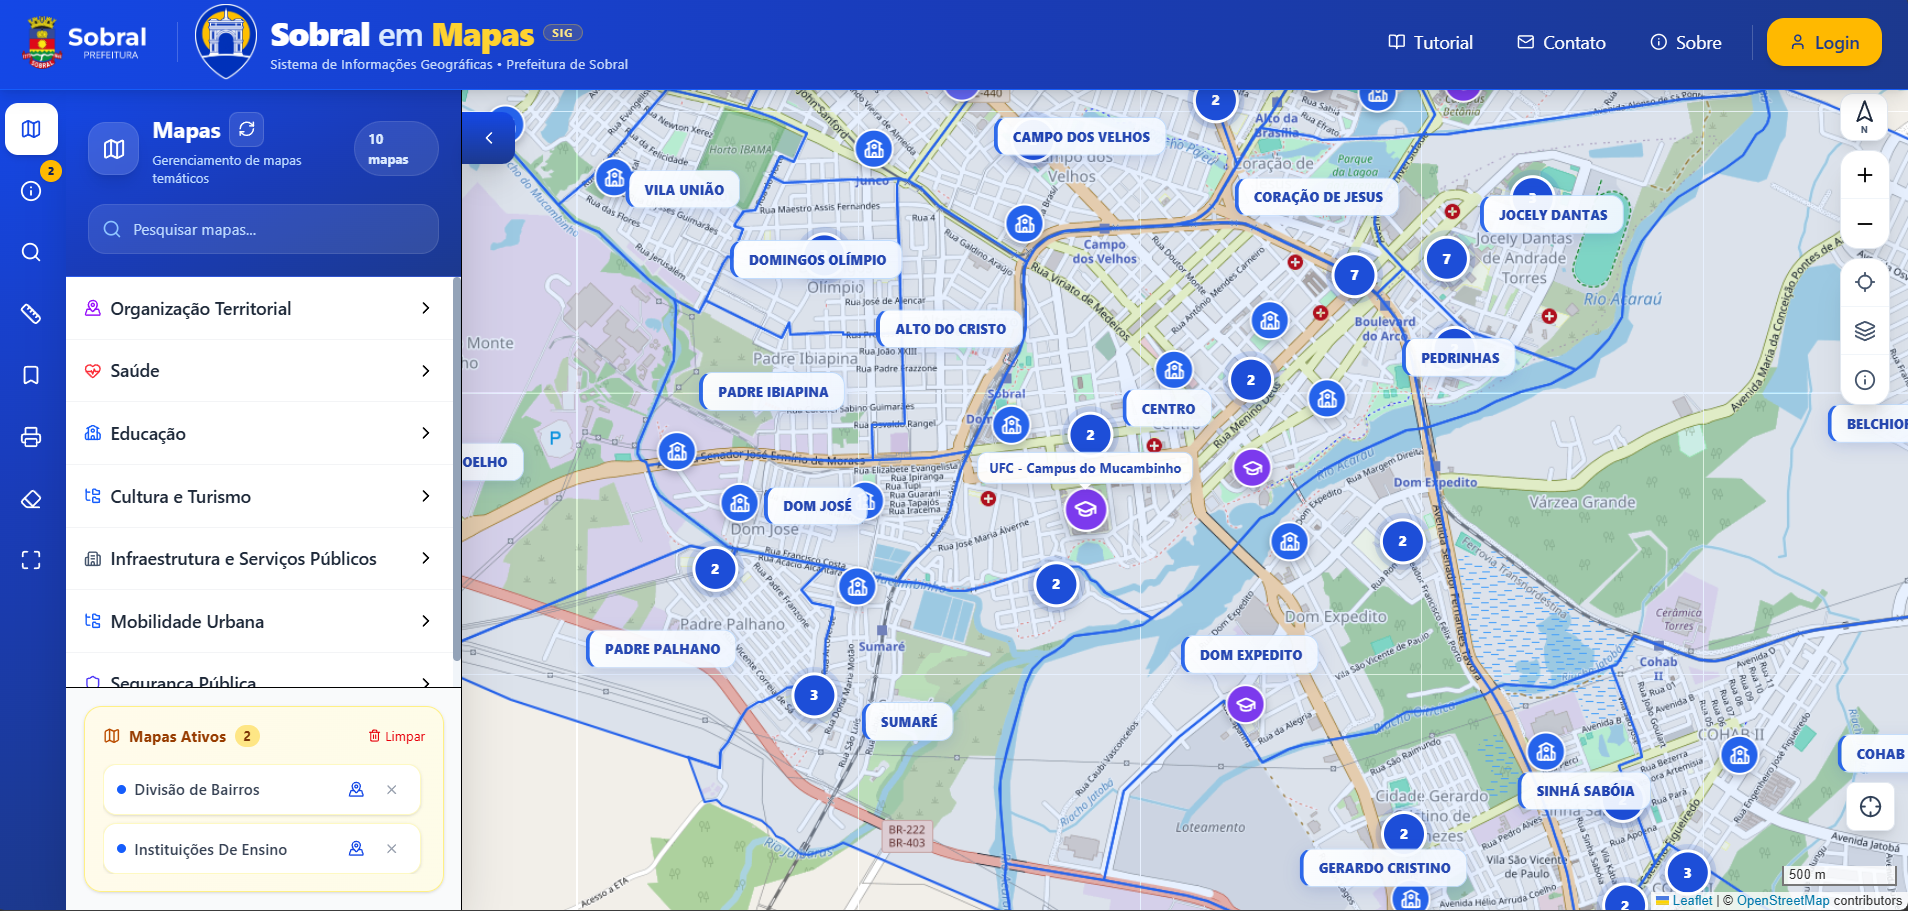
\includegraphics[width=\textwidth]{figuras/interface-principal.png}

    \label{fig:interface-principal}

    \fonte{Elaborado pelo autor.}

\end{figure}

A interface organiza o mapa como elemento central, acompanhado por um cabeçalho, um painel lateral e ferramentas de interação. Na Figura~\ref{fig:interface-principal}, as camadas de bairros e instituições de ensino aparecem simultaneamente, combinando polígonos e marcadores geográficos. A visualização utiliza React e Leaflet, integrados à API Laravel, com suporte a WMS e GeoJSON.

O painel lateral reúne a seleção de camadas, as legendas, a busca de locais, as medições, os favoritos e a impressão. Já os controles sobre o mapa permitem ajustar o zoom, consultar a localização e alternar o mapa-base. Dessa forma, as ferramentas permanecem disponíveis sem interromper a exploração do território.

Para orientar a exploração dos recursos, a plataforma disponibiliza um tutorial interativo acessível pelo cabeçalho, que apresenta as principais ferramentas em etapas e destaca o componente correspondente a cada explicação. Ademais, a página ``Sobre'' reúne informações sobre a proposta do sistema e suas possibilidades de utilização. Esses mecanismos de orientação são acompanhados por ajustes responsivos, de modo que os recursos essenciais permaneçam acessíveis tanto em computadores quanto em dispositivos móveis.

\section{Organização e Visualização das Camadas Temáticas}

\label{sec:visualizacao-camadas}

As informações geoespaciais são agrupadas em categorias e subcategorias, facilitando a localização das camadas. Essa organização é carregada dinamicamente da API Laravel e pode ser atualizada no ambiente administrativo sem exigir alterações no código da interface.

A Figura~\ref{fig:organizacao-camadas} exemplifica essa organização por meio da categoria Educação, da subcategoria Instituições de Ensino e da respectiva camada ativada. No mapa, os estabelecimentos educacionais aparecem como marcadores e rótulos, enquanto o painel de mapas ativos permite acompanhar e remover as camadas selecionadas. Desse modo, a imagem evidencia a integração entre a navegação temática e a visualização cartográfica.

As categorias e subcategorias podem ser expandidas ou recolhidas para reduzir o excesso de informações. Como as camadas são ativadas individualmente, é possível combinar temas e remover os mapas selecionados. Além disso, a ferramenta de enquadramento permite visualizar a extensão geográfica das camadas GeoJSON.

Para facilitar consultas recorrentes, o usuário também pode marcar camadas como favoritas. Já no painel de informações, cada camada ativa apresenta uma legenda associada à sua representação cartográfica. No caso dos arquivos GeoJSON, a simbologia considera o tipo de geometria e as propriedades visuais disponíveis, permitindo ajustes temporários de cor e de exibição dos nomes sem modificar os arquivos originais. Com isso, torna-se mais simples distinguir camadas sobrepostas e adaptar a apresentação dos dados às necessidades de leitura.

\begin{figure}[!htbp]

    \centering

    \caption{Organização temática e seleção de camadas na plataforma Sobral em Mapas}

    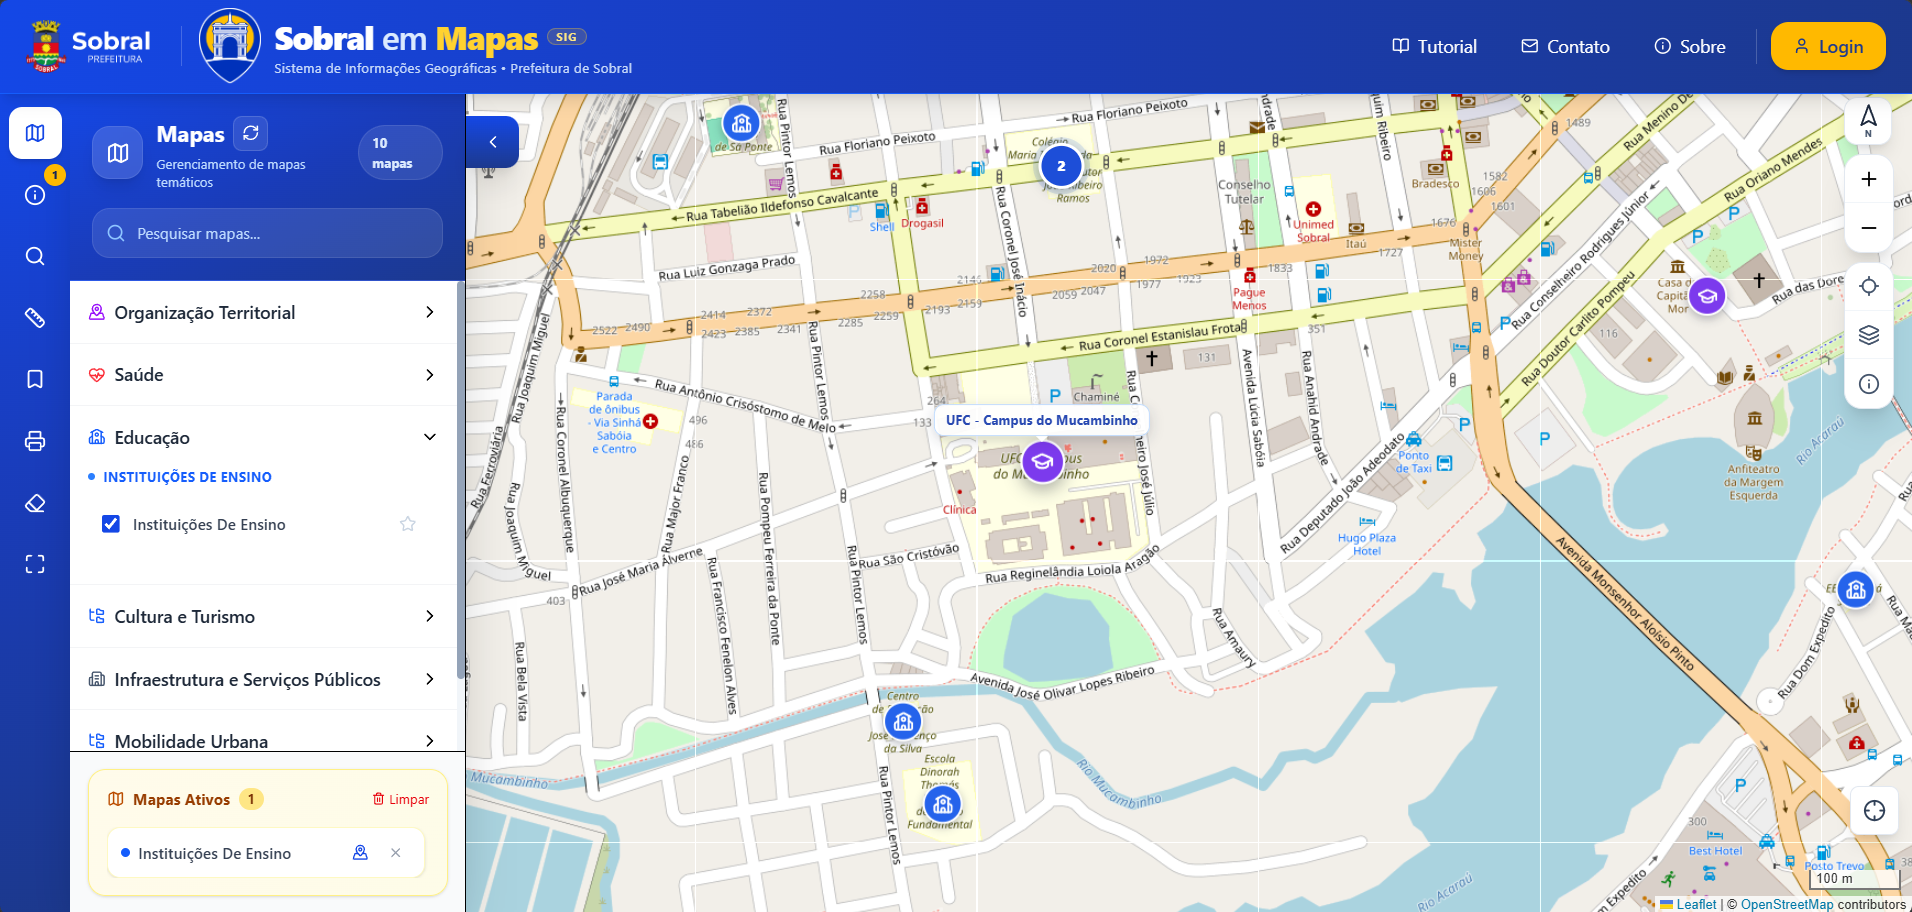
\includegraphics[width=\textwidth]{figuras/organizacao-camadas.png}

    \label{fig:organizacao-camadas}

    \fonte{Elaborado pelo autor.}

\end{figure}

\section{Representação e Consulta de Dados Geoespaciais}

\label{sec:visualizacao-geoespacial}

A plataforma visualiza camadas provenientes de serviços WMS e arquivos GeoJSON, reunindo informações espaciais de diferentes origens. O uso do GeoJSON permite carregar dados vetoriais no navegador e consultar atributos das feições, ampliando as alternativas de disponibilização das informações cartográficas para os usuários.

A Figura~\ref{fig:visualizacao-geoespacial} apresenta a camada Divisão de Distritos por meio de polígonos e rótulos. No painel do distrito Sede, são exibidos atributos como área, nome e identificador, ilustrando a consulta de informações associadas à geometria selecionada.

A consulta às feições GeoJSON ocorre pela seleção de pontos, linhas ou polígonos no mapa. A aplicação apresenta uma janela de informações (\textit{popup}) com título e atributos da feição. Para facilitar a leitura, os campos recebem rótulos claros e as medidas de área e comprimento aparecem em unidades adequadas, sem alterar os valores originais armazenados.

A representação dos pontos utiliza símbolos temáticos definidos pelos atributos das feições, permitindo diferenciar instituições de ensino, serviços de saúde e outros locais. A exibição de ícones e rótulos também varia conforme o nível de zoom, evitando o excesso de elementos em escalas mais afastadas e melhorando a legibilidade.

\begin{figure}[!htbp]

    \centering

    \caption{Visualização da divisão distrital e consulta de atributos geográficos}

    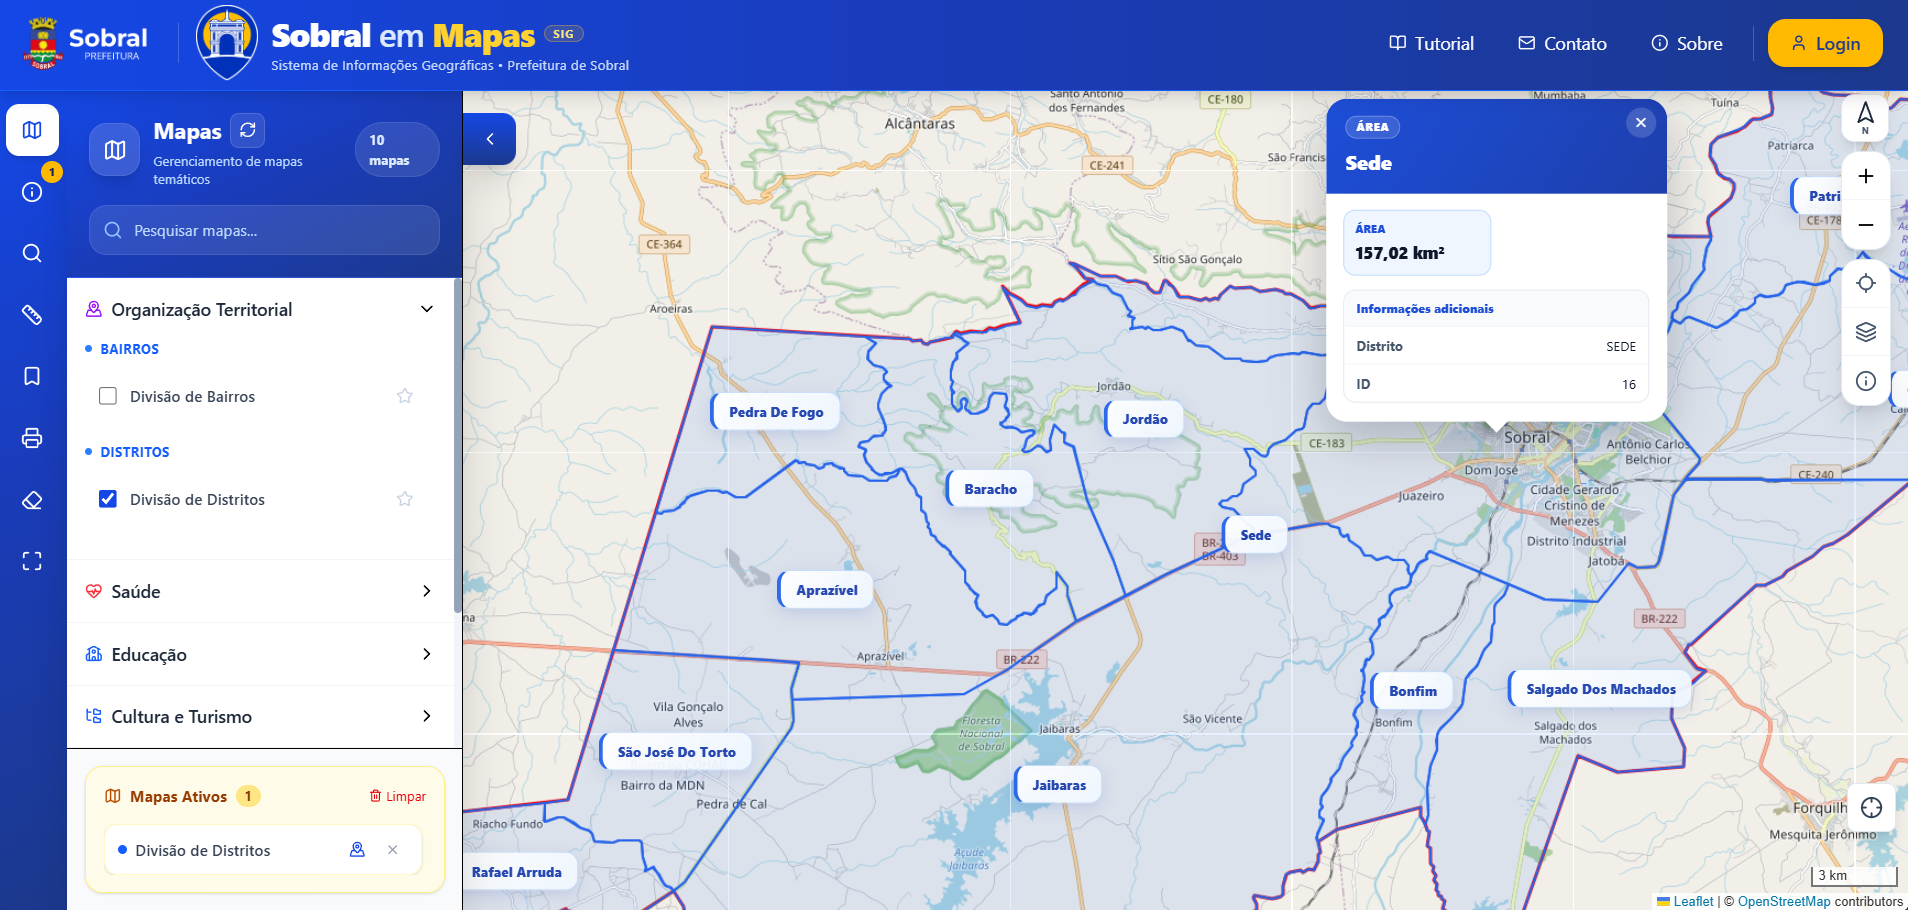
\includegraphics[width=\textwidth]{figuras/visualizacao-geoespacial.png}

    \label{fig:visualizacao-geoespacial}

    \fonte{Elaborado pelo autor.}

\end{figure}

\FloatBarrier

\section{Ferramentas de Interação Cartográfica}

\label{sec:ferramentas-cartograficas}

A plataforma também oferece busca de localizações, medições, favoritos, limpeza do mapa, tela cheia e impressão. Essas ferramentas ampliam a exploração do território e permitem executar operações cartográficas na própria interface, sem recorrer a outros programas.

Na ferramenta de busca, o usuário pode pesquisar endereços, pontos de interesse e coordenadas. O campo sugere locais das camadas GeoJSON e mantém um histórico recente no navegador. Nas consultas externas, um serviço de geocodificação localiza o resultado e centraliza o mapa, exibindo um marcador com informações correspondentes.

As ferramentas de medição permitem desenhar linhas e áreas para obter, respectivamente, distâncias e medidas de superfície. Os resultados são reunidos em um painel no qual os elementos podem ser consultados e excluídos individualmente. Além disso, o usuário pode escolher unidades em metros ou quilômetros para distâncias e em metros quadrados ou quilômetros quadrados para áreas, bem como ajustar cor, espessura e opacidade dos desenhos para diferenciá-los das demais informações cartográficas.

A Figura~\ref{fig:medicao-impressao} apresenta medições e exportação, com uma área de 52.223,15 m² e uma distância de 232,01 m exibidas no painel lateral. Também mostra a seleção de uma região para exportação em PDF, PNG ou JPEG, permitindo compartilhar a visualização do mapa.

Para exportar o mapa, o usuário delimita uma região da visualização por meio de uma área de seleção ajustável e escolhe o formato desejado. A plataforma também permite alternar entre mapas-base, incluindo representações de ruas, imagens de satélite e visualização topográfica, conforme a disponibilidade das fontes configuradas. Dessa maneira, os recursos de exportação se somam aos controles de zoom, localização e tela cheia, oferecendo diferentes formas de explorar o território sem alterar as camadas cadastradas.

\begin{figure}[H]

    \centering

    \caption{Ferramentas de medição e impressão cartográfica da plataforma}

    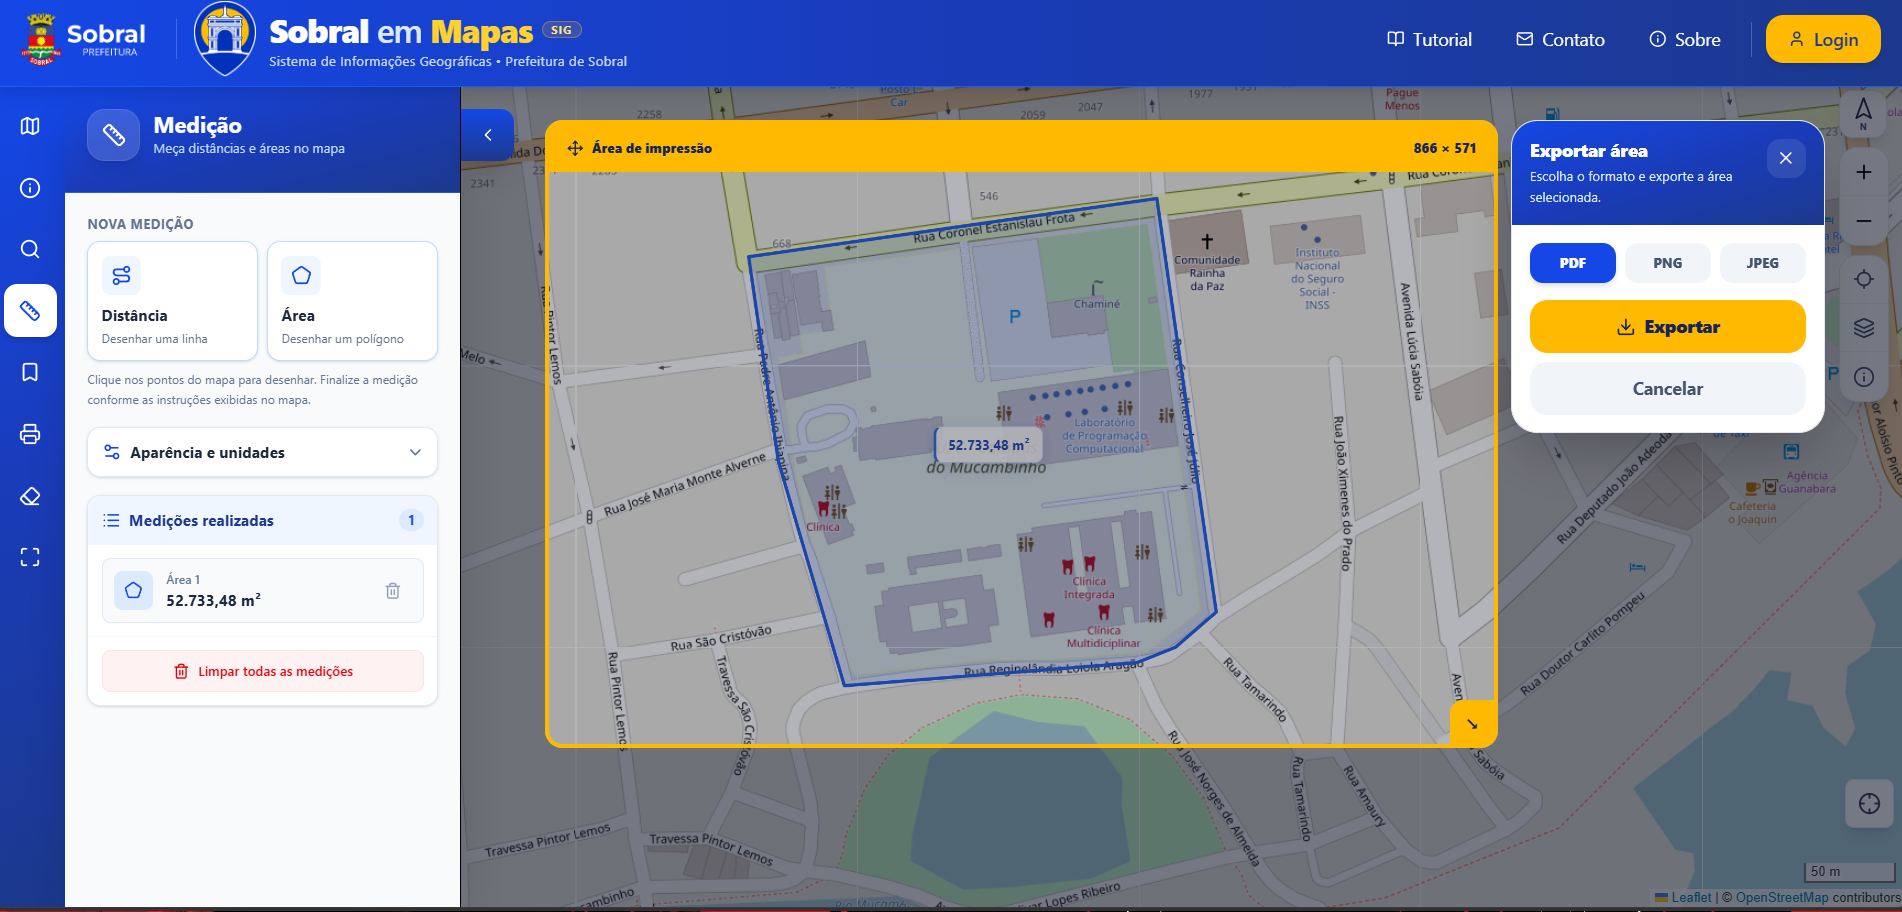
\includegraphics[width=\textwidth]{figuras/medicao-impressao.png}

    \label{fig:medicao-impressao}

    \fonte{Elaborado pelo autor.}

\end{figure}

\section{Ambiente Administrativo da Plataforma}

\label{sec:ambiente-administrativo}

A plataforma dispõe de um ambiente administrativo para gerenciar informações exibidas no mapa. Seu acesso é restrito a usuários autenticados e autorizados, pois reúne operações sobre categorias, subcategorias, camadas, serviços WMS e contas cadastradas. Dessa forma, as funções administrativas permanecem separadas das consultas públicas.

A área administrativa está organizada em páginas de gerenciamento. Enquanto categorias e subcategorias mantêm a organização temática do mapa, as páginas de usuários e solicitações de cadastro permitem acompanhar perfis de acesso e pedidos de aprovação. As operações disponíveis em cada página dependem das permissões do usuário autenticado.

Entre os recursos implementados, destaca-se o gerenciamento de camadas, que permite cadastrar, consultar, editar, ativar, desativar e excluir registros geográficos. A Figura~\ref{fig:gerenciamento-camadas} apresenta a interface correspondente, com indicadores sobre a quantidade de camadas, sua situação de ativação e a visibilidade pública. Além desses indicadores, a página reúne uma tabela com os registros e ferramentas de busca e administração, contemplando tanto camadas associadas a serviços WMS quanto arquivos GeoJSON.

A listagem também apresenta a origem dos dados, sua classificação temática e as condições de publicação de cada camada. Nesse ambiente, a pesquisa textual e os filtros por situação facilitam a localização dos registros, enquanto ações específicas permitem alterar o estado de uma camada, editar seus metadados, excluir o cadastro ou obter o arquivo geográfico, quando disponível. Dessa forma, as operações ficam concentradas em uma interface, e as alterações administrativas podem ser refletidas posteriormente na consulta cartográfica pública.

\begin{figure}[H]

    \centering

    \caption{Interface administrativa de gerenciamento de camadas geográficas}

    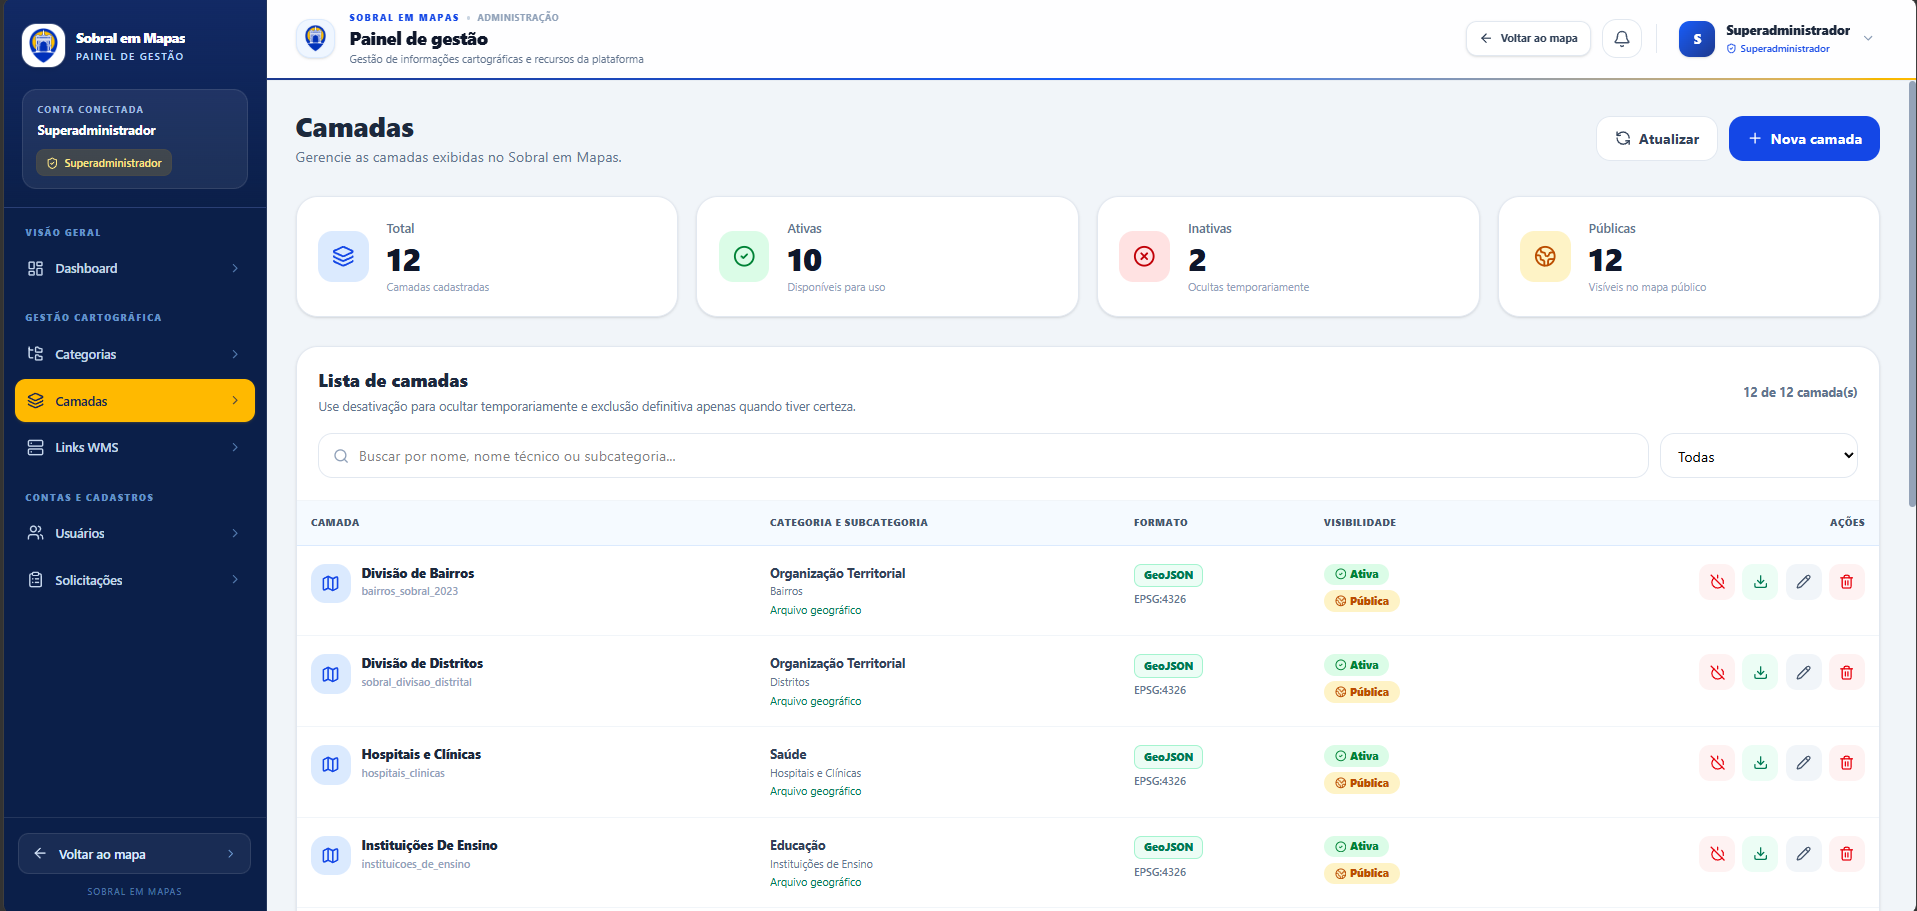
\includegraphics[width=\textwidth]{figuras/gerenciamento-camadas.png}

    \label{fig:gerenciamento-camadas}

    \fonte{Elaborado pelo autor.}

\end{figure}

O cadastro de camadas permite selecionar a fonte cartográfica e informar os metadados necessários à sua organização. Para os arquivos GeoJSON, o formulário oferece a seleção de conteúdos já armazenados ou o envio de novos dados, ambos acompanhados de uma pré-visualização cartográfica. A Figura~\ref{fig:cadastro-geojson} apresenta esse processo com um arquivo de instituições de ensino, permitindo observar sua distribuição espacial antes da conclusão do cadastro.

Para facilitar o cadastro, o formulário organiza em etapas a identificação, a seleção do arquivo e as configurações de apresentação e publicação. Os campos obrigatórios exibem mensagens de validação quando faltam nome, classificação temática ou arquivo geográfico. A biblioteca permite reutilizar arquivos GeoJSON e a pré-visualização mostra seu conteúdo, embora o envio de novas camadas esteja atualmente concentrado nesse formato.

\begin{figure}[H]

    \centering

    \caption{Cadastro de camada GeoJSON com pré-visualização cartográfica}

    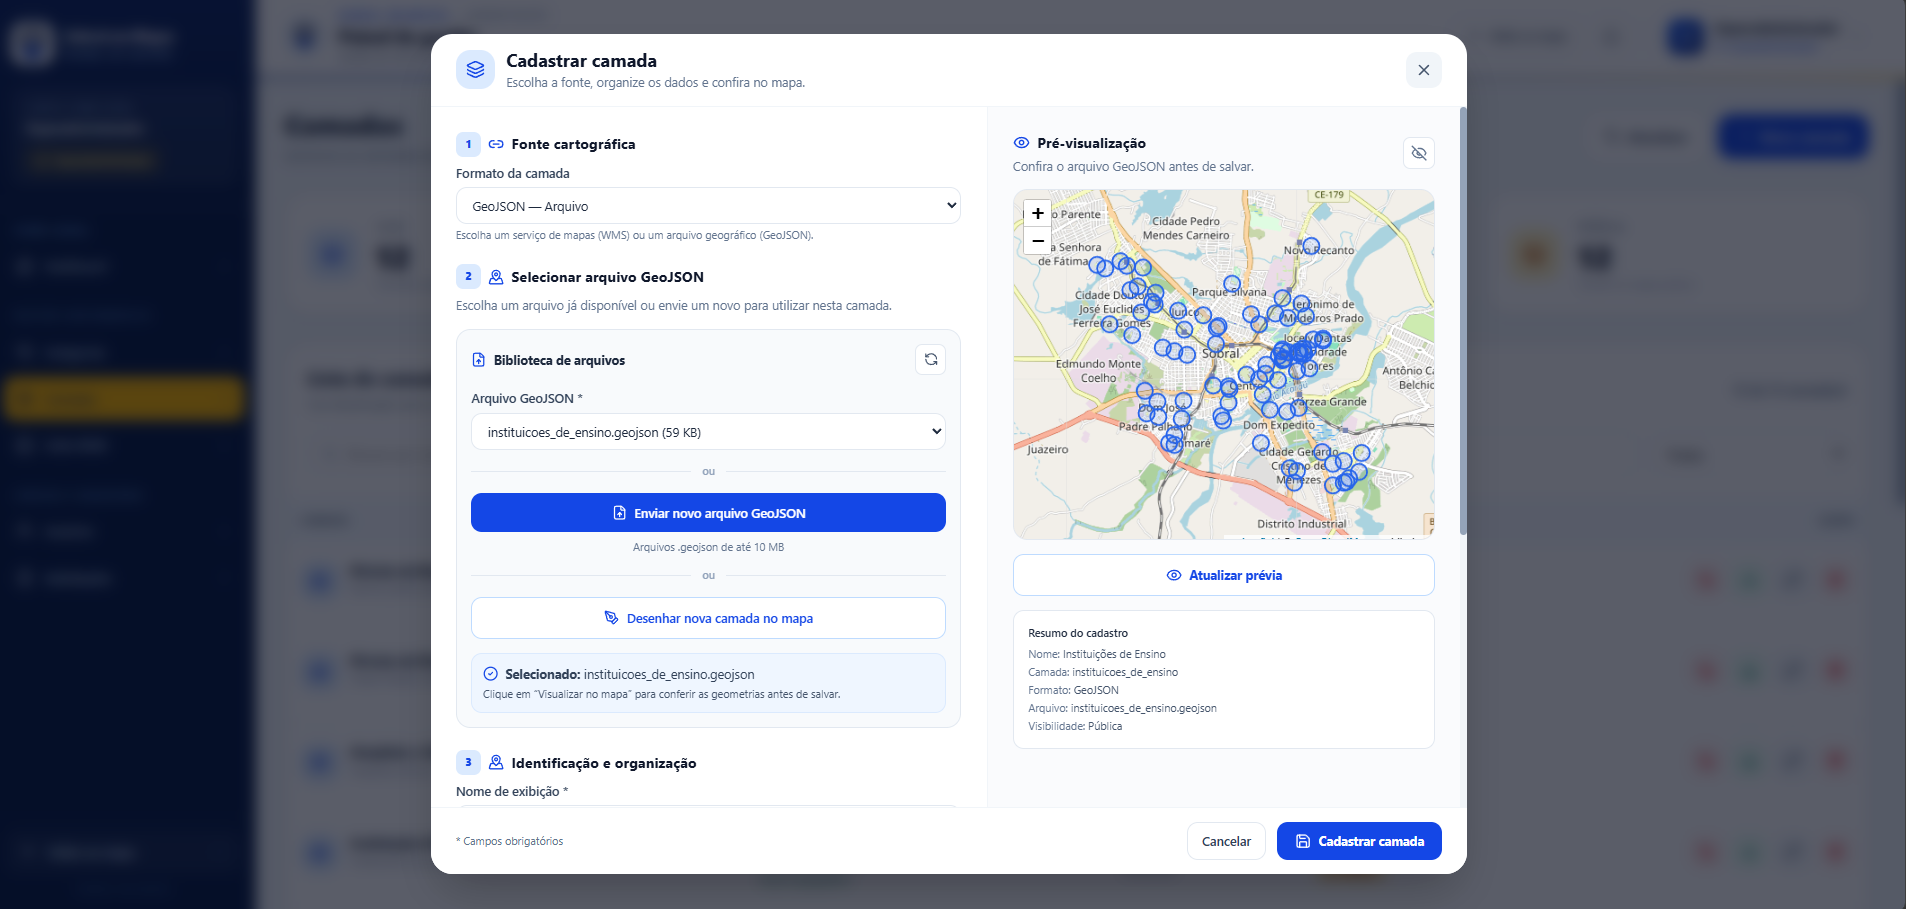
\includegraphics[width=\textwidth]{figuras/cadastro-geojson.png}

    \label{fig:cadastro-geojson}

    \fonte{Elaborado pelo autor.}

\end{figure}

Além do envio de arquivos, foi implementado um editor GeoJSON integrado ao ambiente administrativo, que permite criar e modificar feições no mapa. A ferramenta oferece desenho de pontos, linhas e polígonos, edição de geometrias e ajustes de cor e espessura. A Figura~\ref{fig:editor-geojson} apresenta o editor com instituições de ensino carregadas e seus controles disponíveis.

O editor também oferece opções para desenhar retângulos e círculos, além de editar, excluir, desfazer e refazer operações. Durante a criação das feições, podem ser ajustados cores, estilos de linha, preenchimentos e tamanhos dos pontos, bem como consultadas as medidas das geometrias. Os atributos podem ser alterados antes do salvamento e o conteúdo resultante é convertido para GeoJSON. No caso dos círculos, utiliza-se uma aproximação poligonal, visto que o formato não possui um tipo geométrico específico para representá-los.

\begin{figure}[H]

    \centering

    \caption{Editor de geometrias GeoJSON integrado ao ambiente administrativo}

    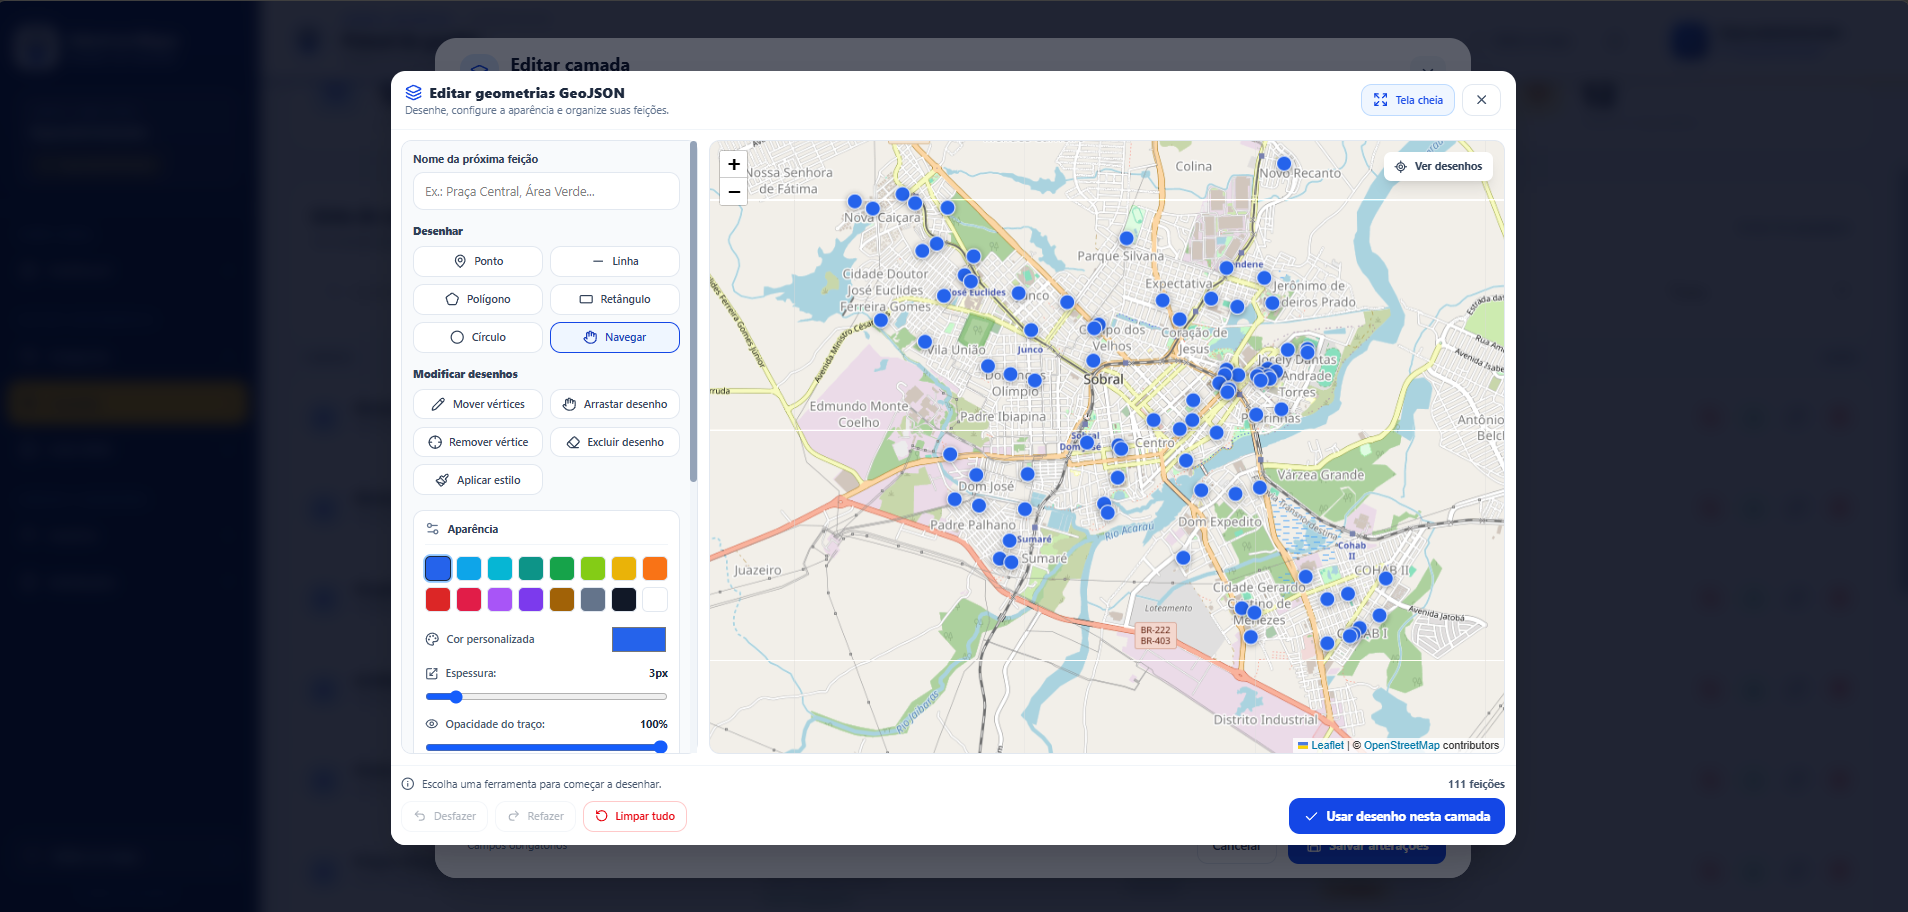
\includegraphics[width=\textwidth]{figuras/editor-geojson.png}

    \label{fig:editor-geojson}

    \fonte{Elaborado pelo autor.}

\end{figure}

Esses recursos ampliam o gerenciamento geográfico por permitir incorporar arquivos vetoriais e editar geometrias na plataforma. Assim, o ambiente administrativo organiza as camadas e disponibiliza suas informações na interface pública.

\section{Implantação e Ambiente de Execução}

\label{sec:implantacao-ambiente-execucao}

Após a integração das funcionalidades, o ``Sobral em Mapas'' foi disponibilizado em nuvem com cliente cartográfico e servidor separados. O \textit{front-end}, desenvolvido em React, foi publicado na Vercel a partir do processo de compilação do Vite. Já o \textit{back-end}, em Laravel, foi implantado no Railway para executar a API. Os componentes se comunicam por endereços definidos em variáveis de ambiente e podem ser atualizados de maneira independente.

Para o desenvolvimento e a execução local, foi utilizado o Docker, que organiza o servidor de aplicação, o banco de dados e os serviços auxiliares em contêineres. Essa configuração contribui para a padronização do ambiente, facilitando as atividades de desenvolvimento e verificação do sistema. A Figura~\ref{fig:implantacao-ambientes} apresenta os três ambientes utilizados, reunindo a publicação da interface na Vercel, a execução da API no Railway e a organização dos contêineres no Docker.

\begin{figure}[H]

    \centering

    \caption{Ambientes de publicação e execução da plataforma Sobral em Mapas}

    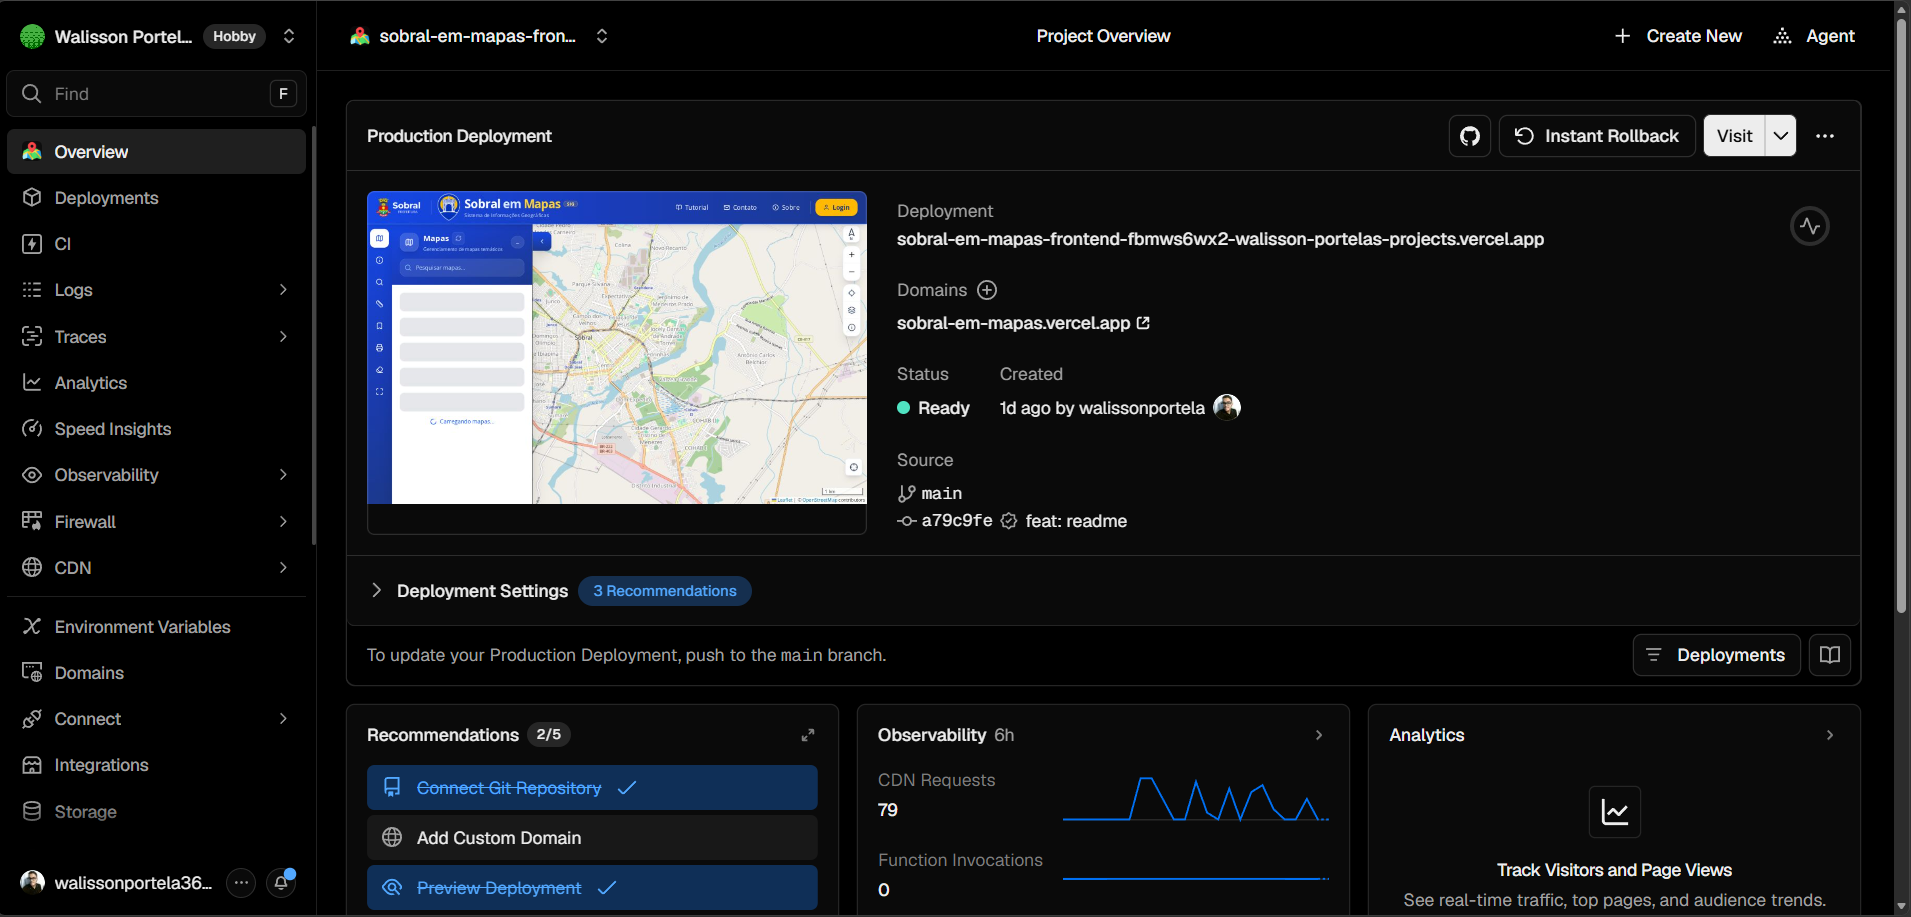
\includegraphics[width=1.0\textwidth,height=0.25\textheight,keepaspectratio]{figuras/implantacao-vercel.png}

    \par\smallskip

    {\footnotesize (a) Publicação do \textit{front-end} na Vercel}

    \par\medskip

    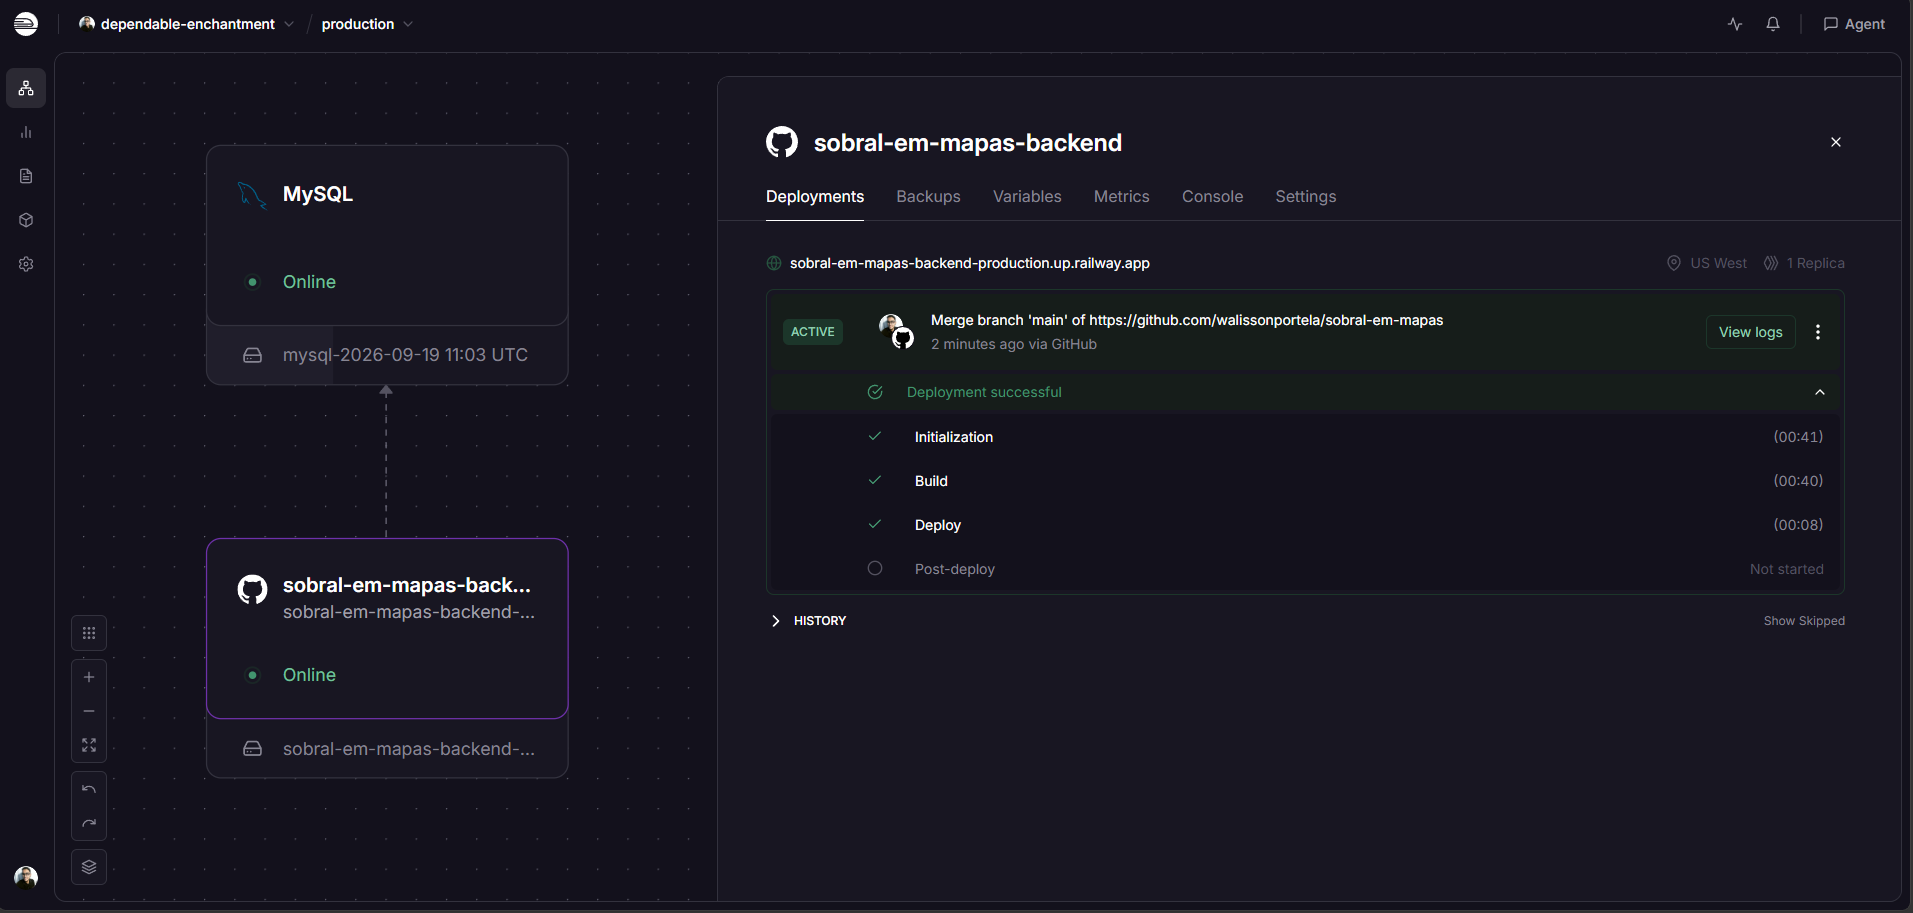
\includegraphics[width=1.0\textwidth,height=0.25\textheight,keepaspectratio]{figuras/implantacao-railway.png}

    \par\smallskip

    {\footnotesize (b) Execução da API no Railway}

    \par\medskip

    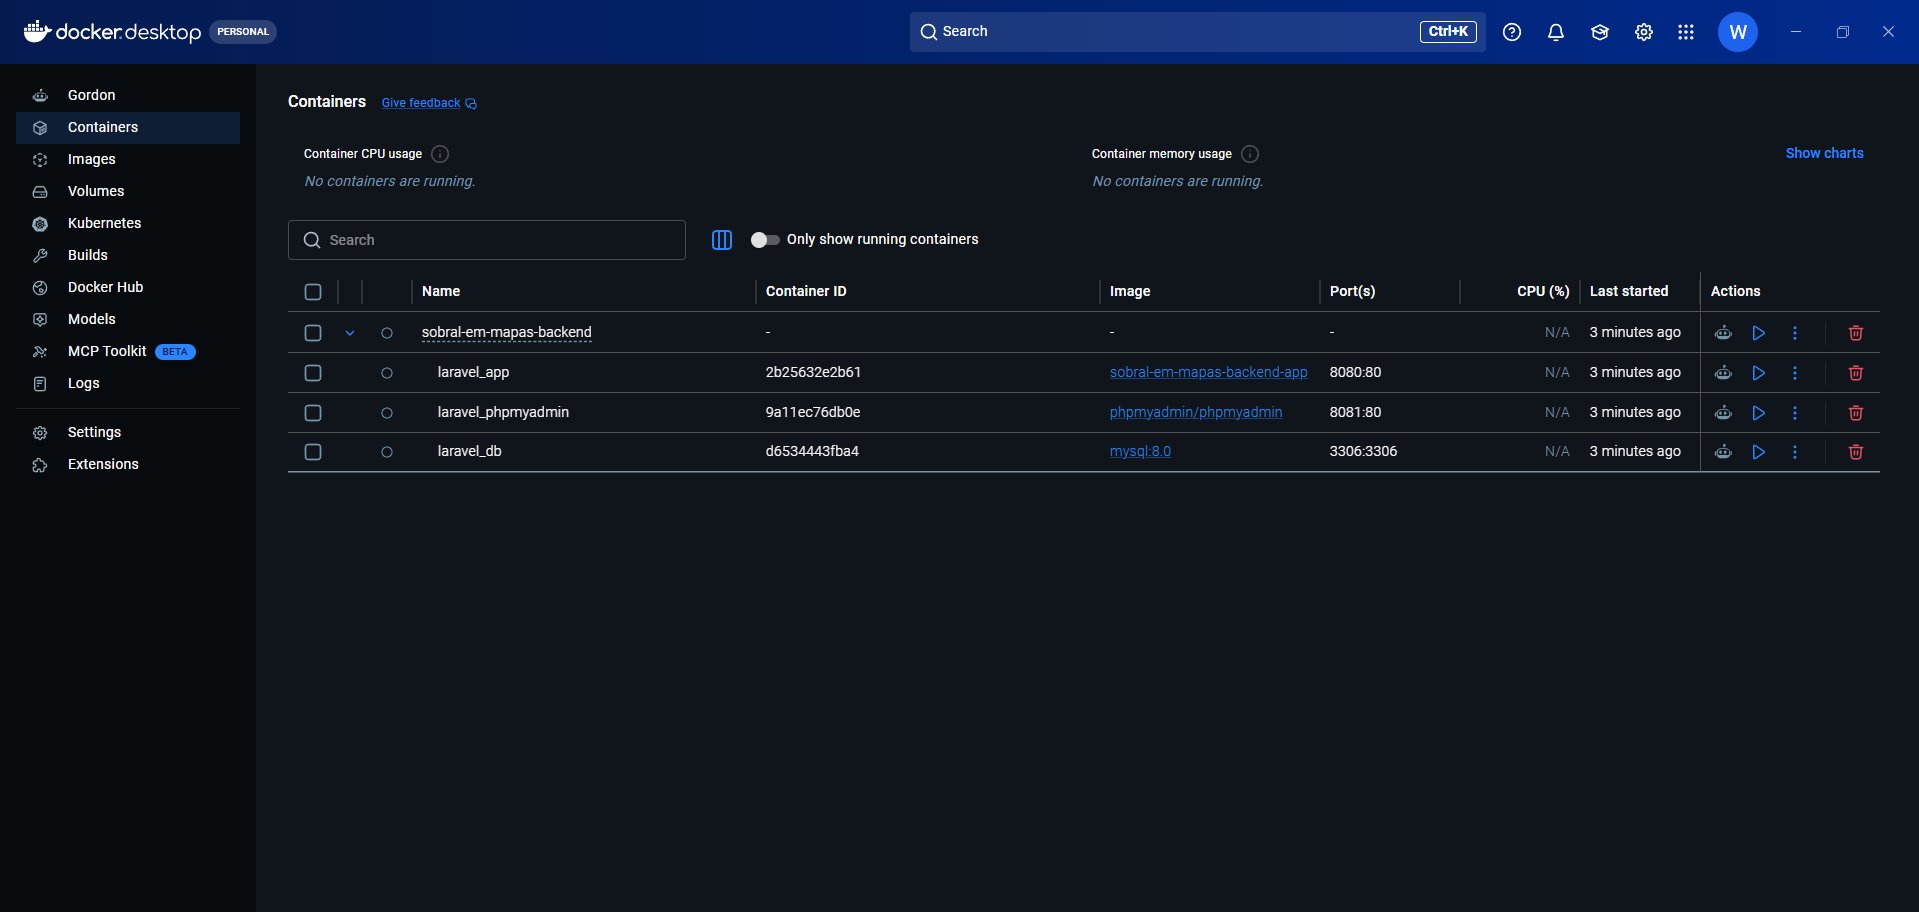
\includegraphics[width=1.20\textwidth,height=0.25\textheight,keepaspectratio]{figuras/implantacao-docker.png}

    \par\smallskip

    {\footnotesize (c) Ambiente local conteinerizado com Docker}

    \label{fig:implantacao-ambientes}

    \fonte{Capturas de tela realizadas pelo autor.}

\end{figure}

A utilização desses ambientes evidencia a separação entre a publicação da interface, a execução dos serviços administrativos e a preparação do ambiente local. Embora essa organização contribua para a disponibilização e a manutenção da plataforma, algumas limitações permanecem relacionadas à infraestrutura. Entre elas, destaca-se a dependência do GeoServer para o consumo dos serviços WMS, parcialmente contornada pela incorporação de arquivos GeoJSON como fonte adicional de dados geográficos. Além disso, a persistência desses arquivos exige configurações adequadas de armazenamento no ambiente de hospedagem.

\FloatBarrier

\section{Atendimento aos Requisitos}

\label{sec:atendimento-requisitos}

A análise do atendimento aos requisitos considerou as funcionalidades implementadas e os procedimentos de verificação descritos na Metodologia. Os resultados evidenciam a implementação dos principais recursos previstos, abrangendo a visualização cartográfica, as ferramentas de interação, o gerenciamento administrativo e a integração entre diferentes fontes geoespaciais. Para relacionar essas entregas ao planejamento do sistema, a Tabela~\ref{tab:atendimento-requisitos} apresenta os requisitos funcionais e seus respectivos recursos implementados.

\begin{table}[H]

    \captionsetup{width=15cm}

    \Caption{\label{tab:atendimento-requisitos} Relação entre requisitos funcionais e funcionalidades implementadas}

    \IBGEtab{}{

        \begin{tabular}{p{1.6cm}p{12.8cm}}

            \toprule

            \textbf{Código} &

            \textbf{Funcionalidade implementada} \\

            \midrule \midrule

            RF01 &

            Interface cartográfica interativa com camadas organizadas por categorias e subcategorias. \\

            \midrule

            RF02 &

            Pesquisa, ativação e desativação de camadas, com consulta às informações geográficas associadas. \\

            \midrule

            RF03 &

            Pesquisa de endereços e pontos de interesse, com localização dos resultados no mapa. \\

            \midrule

            RF04 &

            Ferramentas de medição de distâncias e áreas, além da criação, edição e armazenamento de geometrias GeoJSON no ambiente administrativo. \\

            \midrule

            RF05 &

            Recursos de favoritos, limpeza do mapa, tela cheia e impressão ou exportação cartográfica. \\

            \midrule

            RF06 &

            Formulário de contato integrado à API para encaminhamento de mensagens. \\

            \midrule

            RF07 &

            Cadastro, autenticação e controle de acesso conforme os perfis e a situação de aprovação dos usuários. \\

            \midrule

            RF08 &

            Gerenciamento administrativo de usuários, perfis de acesso e solicitações de aprovação. \\

            \midrule

            RF09 &

            Cadastro e manutenção de categorias e subcategorias utilizadas na organização das camadas. \\

            \midrule

            RF10 &

            Gerenciamento de camadas WMS e GeoJSON, incluindo metadados, envio de arquivos e pré-visualização cartográfica. \\

            \bottomrule

        \end{tabular}

    }{

        \Fonte{Elaborado pelo autor.}

    }

\end{table}

Os requisitos não funcionais contemplam responsividade, separação de responsabilidades, integração com WMS e GeoJSON, autenticação, autorização e validação de dados. Também foram utilizados componentes React reutilizáveis, comunicação HTTP/HTTPS, Docker e variáveis de ambiente. Essas decisões atendem a aspectos técnicos previstos, embora segurança, desempenho e responsividade ainda exijam testes em diferentes condições.

De modo geral, foram implementadas as principais funcionalidades previstas. O suporte a arquivos GeoJSON permite disponibilizar camadas sem depender apenas dos serviços WMS externos, reduzindo os efeitos das limitações dessa infraestrutura.

\section{Avaliação com Usuários}

\label{sec:avaliacao-usuarios}

Para complementar as verificações funcionais, foi iniciada uma avaliação exploratória de usabilidade, na qual participantes convidados executam atividades na interface pública e no ambiente administrativo do ``Sobral em Mapas''. Após a consulta às camadas, a utilização das ferramentas cartográficas e as operações de gerenciamento orientadas por um guia de teste, os participantes foram convidados a responder voluntariamente a um questionário eletrônico sobre facilidade de uso, compreensão das informações e experiência geral.

\section{Discussão dos Resultados e Limitações}

\label{sec:discussao-resultados}

Os resultados apresentados demonstram a implementação de uma plataforma WebGIS que reúne recursos de consulta, visualização e gerenciamento de informações geoespaciais do município de Sobral. A organização temática das camadas, as ferramentas cartográficas e o ambiente administrativo evidenciam a integração entre os componentes desenvolvidos. Além disso, a separação entre \textit{front-end}, \textit{back-end} e fontes de dados contribuiu para estruturar a solução e incorporar novas funcionalidades ao longo do desenvolvimento.

Entre os resultados obtidos, destaca-se a ampliação do suporte a dados geoespaciais por meio do formato GeoJSON, que permite incorporar arquivos vetoriais, consultar atributos e criar ou editar geometrias no ambiente administrativo. Dessa forma, a plataforma passou a oferecer uma alternativa complementar aos serviços WMS, reduzindo a dependência exclusiva de infraestrutura externa para disponibilizar camadas cartográficas.

Entretanto, algumas limitações permanecem associadas à arquitetura adotada, visto que o consumo de camadas WMS depende da disponibilidade dos serviços fornecidos pelo GeoServer, enquanto os arquivos GeoJSON exigem armazenamento e persistência adequados no servidor de aplicação. Ademais, o processamento de conjuntos geográficos extensos diretamente no navegador pode afetar o desempenho, sobretudo em dispositivos com recursos computacionais limitados, aspecto que ainda demanda verificações específicas.

Embora as funcionalidades implementadas indiquem a viabilidade técnica da solução, são necessárias avaliações com diferentes perfis de usuários. As verificações funcionais oferecem evidências do comportamento dos recursos, enquanto a avaliação com usuários, ainda em coleta, deverá identificar percepções de usabilidade e dificuldades de interação.
    
\chapter{Conclusões e Trabalhos Futuros}
\label{chap:conclusoes-e-trabalhos-futuros}

O presente trabalho teve como objetivo desenvolver a plataforma WebGIS ``Sobral em Mapas'', destinada à organização, ao gerenciamento e à visualização de dados geoespaciais do município de Sobral, no Ceará. Para isso, foram aplicados conceitos de Engenharia de Software, desde o levantamento de requisitos e a modelagem dos dados até a implementação de uma arquitetura desacoplada, utilizando React e Leaflet no \textit{front-end}, Laravel no \textit{back-end} e MySQL na persistência administrativa. Como resultado, foi desenvolvida uma aplicação \textit{web} funcional que reúne ferramentas cartográficas e recursos administrativos para consultar informações territoriais, gerenciar camadas temáticas e controlar o acesso dos usuários.

Entre as principais contribuições, destaca-se a integração de diferentes fontes geoespaciais, inicialmente baseada nos serviços WMS do GeoServer e posteriormente ampliada para arquivos GeoJSON. Essa adaptação reduziu a dependência exclusiva de serviços externos, possibilitando o envio, a pré-visualização e a criação de geometrias diretamente na plataforma. Também foram implementadas ferramentas de pesquisa, medição, exportação e personalização cartográfica, enquanto o uso do Docker no ambiente local e a implantação independente do \textit{front-end} e do \textit{back-end} contribuíram para a organização e a padronização da execução dos componentes. Dessa forma, os resultados demonstram a viabilidade técnica de integrar gerenciamento administrativo e visualização geoespacial em uma plataforma voltada à gestão municipal e à consulta integrada de informações sobre o território.

Além das verificações funcionais, foi realizada uma avaliação exploratória de usabilidade com usuários voluntários, cujos resultados indicaram uma percepção favorável quanto à facilidade de utilização, à satisfação e à utilidade da plataforma. A avaliação também permitiu identificar dificuldades pontuais, especialmente nas operações administrativas de gerenciamento de camadas, contribuindo para orientar ajustes na interface e reconhecer oportunidades de aprimoramento. Embora os resultados tenham sido positivos, o caráter exploratório do estudo e o número limitado de participantes indicam a necessidade de avaliações complementares com diferentes perfis de usuários, incluindo profissionais e gestores públicos.

Apesar dos avanços alcançados, permanecem limitações relacionadas à disponibilidade dos serviços WMS externos, à necessidade de armazenamento persistente dos arquivos GeoJSON no ambiente de hospedagem e ao processamento de conjuntos extensos de dados geográficos. Esses aspectos poderão ser aprimorados por meio de melhorias na infraestrutura, mecanismos de \textit{cache}, simplificação de geometrias e carregamento progressivo de camadas, favorecendo o desempenho e a disponibilidade da plataforma em diferentes condições de utilização.

Como trabalhos futuros, propõe-se ampliar o suporte a formatos geográficos, como KML, e a serviços baseados no padrão WFS, além de incorporar filtros mais detalhados sobre os atributos das camadas e ferramentas adicionais de análise espacial. Também se pretende aprimorar o acompanhamento da origem e da atualização das informações geográficas, favorecendo a organização, a interoperabilidade e a confiabilidade dos dados disponibilizados. Essas melhorias poderão ampliar as possibilidades de utilização da plataforma em atividades de consulta, planejamento e gestão territorial.

Outra possibilidade de evolução consiste no desenvolvimento de uma versão móvel do ``Sobral em Mapas'', com recursos de consulta cartográfica, geolocalização e acesso a informações selecionadas em situações de baixa conectividade. Essa iniciativa poderá começar pela implementação de uma \textit{Progressive Web App} (PWA) ou avançar para uma aplicação desenvolvida com React Native, aproveitando os conhecimentos e a lógica de integração já utilizados no projeto. Também se considera a integração de um assistente virtual (\textit{chatbot}), utilizando tecnologias como o \textit{framework} Rasa para interpretar perguntas em linguagem natural, orientar os usuários e facilitar o acesso às ferramentas e camadas do mapa. Ademais, pretende-se dar continuidade às melhorias de acessibilidade, responsividade e personalização da interface, considerando as necessidades identificadas em futuras avaliações.

Conclui-se, portanto, que o ``Sobral em Mapas'' alcançou seu objetivo principal ao reunir visualização cartográfica e gerenciamento administrativo em uma plataforma WebGIS funcional. A arquitetura desacoplada e o suporte a diferentes fontes geoespaciais estabeleceram uma base tecnológica que favorece a manutenção e a evolução do sistema, enquanto a avaliação exploratória apresentou indícios favoráveis de sua aceitação pelos participantes. Assim, a plataforma demonstra potencial para contribuir com a organização e a disponibilização de informações territoriais, oferecendo recursos que podem apoiar consultas públicas e atividades de planejamento e gestão do município de Sobral.

    
    % --- Pós-textuais ---
    \bibliography{3-pos-textuais/referencias}
    
    % Descomente abaixo caso tenha apêndices ou anexos
    %\imprimirapendices
    %    \apendice{Questionário de Avaliação de Usabilidade da Plataforma Sobral em Mapas}
\label{ap:questionario-usabilidade}

Este apêndice apresenta o conteúdo do questionário eletrônico utilizado na avaliação exploratória de usabilidade da plataforma ``Sobral em Mapas'', elaborado no Google Forms e disponibilizado aos participantes após a realização das atividades propostas no guia de teste. O instrumento reúne questões sobre experiência prévia, utilização das ferramentas cartográficas, gerenciamento administrativo, percepção geral da plataforma e dificuldades encontradas. A participação foi voluntária, e as respostas foram destinadas à análise agrupada para fins acadêmicos.

% Apresentação compacta das alternativas de múltipla escolha.
\newenvironment{alternativasFormulario}
{\begin{itemize}\renewcommand{\labelitemi}{$\circ$}\setlength{\itemsep}{1pt}\setlength{\parsep}{0pt}}
{\end{itemize}}

% Repete, em cada afirmação, as cinco opções da escala utilizada no Forms.
% Os pontos intermediários não recebiam rótulos no formulário original.
\newcommand{\escalaFormulario}{%
    \par\noindent\hspace*{0.8cm}%
    {\small $\circ$~1\qquad $\circ$~2\qquad $\circ$~3\qquad $\circ$~4\qquad $\circ$~5}%
    \par\medskip
}

% Mantém cada afirmação junto das opções da escala.
\newcommand{\questaoComEscala}[2]{%
    \par\noindent\begin{minipage}{\linewidth}
    \noindent\textbf{Questão #1.} #2
    \escalaFormulario
    \end{minipage}
    \par\medskip
}

\noindent\textbf{Consentimento para participação}
\par\medskip

\noindent\textbf{Questão 1.} Você concorda em participar voluntariamente desta pesquisa, sabendo que suas respostas serão utilizadas para fins acadêmicos?
\begin{alternativasFormulario}
    \item Sim, concordo em participar.
    \item Não, prefiro não participar.
\end{alternativasFormulario}

\noindent\textbf{Perfil do Participante}
\par\medskip

\noindent\textbf{Questão 2.} Qual é sua experiência prévia com mapas digitais e ferramentas de geoprocessamento?
\begin{alternativasFormulario}
    \item Nunca utilizei mapas digitais.
    \item Já utilizei mapas digitais, como Google Maps.
    \item Já utilizei plataformas de mapas temáticos ou WebGIS.
    \item Já utilizei ferramentas de geoprocessamento, como QGIS.
\end{alternativasFormulario}

\noindent\textbf{Questão 3.} Qual dispositivo você utilizou para realizar o teste?
\begin{alternativasFormulario}
    \item Computador ou notebook.
    \item Celular.
    \item Tablet.
\end{alternativasFormulario}

\noindent\textbf{Avaliação do Mapa e das Ferramentas}
\par\medskip

Considerando a experiência ao explorar o mapa sem realizar login, as questões 4 a 6 utilizaram uma escala de concordância de 1 a 5, na qual 1 corresponde a ``Discordo totalmente'' e 5 corresponde a ``Concordo totalmente''.

\medskip
\questaoComEscala{4}{Foi fácil compreender a organização da interface e encontrar as principais funcionalidades do mapa.}

\questaoComEscala{5}{Foi fácil localizar, selecionar e ativar as camadas geográficas disponíveis na plataforma.}

\questaoComEscala{6}{As informações apresentadas nas camadas geográficas foram claras e fáceis de compreender.}

\noindent\textbf{Avaliação do Ambiente Administrativo}
\par\medskip

Considerando a experiência com o gerenciamento de camadas geográficas, as questões 7 e 8 utilizaram a mesma escala de concordância de 1 a 5, de ``Discordo totalmente'' a ``Concordo totalmente''.

\medskip
\questaoComEscala{7}{Foi fácil acessar o ambiente administrativo e localizar as funcionalidades de gerenciamento de camadas.}

\questaoComEscala{8}{O processo de cadastrar, editar e excluir uma camada geográfica foi simples e intuitivo.}

\noindent\textbf{Questão 9.} Como você criou a camada durante o teste?
\begin{alternativasFormulario}
    \item Utilizei o arquivo GeoJSON disponibilizado no Google Drive.
    \item Desenhei uma nova camada diretamente no mapa.
    \item Não consegui concluir o cadastro da camada.
\end{alternativasFormulario}

\noindent\textbf{Avaliação Geral da Plataforma}
\par\medskip

Considerando toda a experiência com o ``Sobral em Mapas'', as questões 10 a 13 utilizaram a escala de concordância de 1 a 5, na qual 1 representa ``Discordo totalmente'' e 5 representa ``Concordo totalmente''.

\medskip
\questaoComEscala{10}{De modo geral, considero a plataforma Sobral em Mapas fácil de utilizar.}

\questaoComEscala{11}{Considero o Sobral em Mapas uma ferramenta útil para consultar e organizar informações geográficas do município.}

\questaoComEscala{12}{De modo geral, fiquei satisfeito(a) com minha experiência ao utilizar o Sobral em Mapas.}

\questaoComEscala{13}{Eu utilizaria o Sobral em Mapas novamente caso precisasse consultar ou gerenciar informações geográficas de Sobral.}

\noindent\textbf{Dificuldades e Sugestões}
\par\medskip

\noindent\textbf{Questão 14.} Você conseguiu concluir as atividades propostas no guia de teste?
\begin{alternativasFormulario}
    \item Sim, concluí todas as atividades sem dificuldades.
    \item Sim, concluí todas, mas encontrei algumas dificuldades.
    \item Consegui concluir apenas uma parte das atividades.
    \item Não consegui concluir as atividades.
\end{alternativasFormulario}

\noindent\textbf{Questão 15.} Em qual etapa você encontrou maior dificuldade durante o teste?
\begin{alternativasFormulario}
    \item Explorar o mapa e ativar camadas.
    \item Utilizar as ferramentas cartográficas.
    \item Acessar e navegar no ambiente administrativo.
    \item Cadastrar uma camada.
    \item Editar ou excluir uma camada.
    \item Não encontrei dificuldades significativas.
\end{alternativasFormulario}

\noindent\textbf{Questão 16.} Você tem alguma sugestão de melhoria ou comentário sobre sua experiência com o Sobral em Mapas? (Opcional)

\medskip
\noindent\textbf{\textit{Questão opcional de resposta aberta.}}

    %\imprimiranexos
    %    \anexo{Exemplo de um anexo}
\label{an:ex_anexo_a}

Um anexo é um documento que não foi elaborado pelo autor, ou seja, o autor apenas anexa. Anexos podem ser tabelas, mapas, diagramas, \textit{datasheets}, manuais e etc. 



       

\end{document}